\documentclass[a4paper,
fontsize=11pt,
%headings=small,
oneside,
numbers=noperiodatend,
parskip=half-,
bibliography=totoc,
final
]{scrartcl}

\usepackage[babel]{csquotes}
\usepackage{synttree}
\usepackage{graphicx}
\setkeys{Gin}{width=.4\textwidth} %default pics size

\graphicspath{{./plots/}}
\usepackage[ngerman]{babel}
\usepackage[T1]{fontenc}
%\usepackage{amsmath}
\usepackage[utf8x]{inputenc}
\usepackage [hyphens]{url}
\usepackage{booktabs} 
\usepackage[left=2.4cm,right=2.4cm,top=2.3cm,bottom=2cm,includeheadfoot]{geometry}
\usepackage{eurosym}
\usepackage{multirow}
\usepackage[ngerman]{varioref}
\setcapindent{1em}
\renewcommand{\labelitemi}{--}
\usepackage{paralist}
\usepackage{pdfpages}
\usepackage{lscape}
\usepackage{float}
\usepackage{acronym}
\usepackage{eurosym}
\usepackage{longtable,lscape}
\usepackage{mathpazo}
\usepackage[normalem]{ulem} %emphasize weiterhin kursiv
\usepackage[flushmargin,ragged]{footmisc} % left align footnote
\usepackage{ccicons} 
\setcapindent{0pt} % no indentation in captions

%%%% fancy LIBREAS URL color 
\usepackage{xcolor}
\definecolor{libreas}{RGB}{112,0,0}

\usepackage{listings}

\urlstyle{same}  % don't use monospace font for urls

\usepackage[fleqn]{amsmath}

%adjust fontsize for part

\usepackage{sectsty}
\partfont{\large}

%Das BibTeX-Zeichen mit \BibTeX setzen:
\def\symbol#1{\char #1\relax}
\def\bsl{{\tt\symbol{'134}}}
\def\BibTeX{{\rm B\kern-.05em{\sc i\kern-.025em b}\kern-.08em
    T\kern-.1667em\lower.7ex\hbox{E}\kern-.125emX}}

\usepackage{fancyhdr}
\fancyhf{}
\pagestyle{fancyplain}
\fancyhead[R]{\thepage}

% make sure bookmarks are created eventough sections are not numbered!
% uncommend if sections are numbered (bookmarks created by default)
\makeatletter
\renewcommand\@seccntformat[1]{}
\makeatother

% typo setup
\clubpenalty = 10000
\widowpenalty = 10000
\displaywidowpenalty = 10000

\usepackage{hyperxmp}
\usepackage[colorlinks, linkcolor=black,citecolor=black, urlcolor=libreas,
breaklinks= true,bookmarks=true,bookmarksopen=true]{hyperref}
\usepackage{breakurl}

%meta
%meta

\fancyhead[L]{V. de Toledo, F. Garcês\\ %author
LIBREAS. Library Ideas, 40 (2021). % journal, issue, volume.
\href{http://nbn-resolving.de/}
{}} % urn 
% recommended use
%\href{http://nbn-resolving.de/}{\color{black}{urn:nbn:de...}}
\fancyhead[R]{\thepage} %page number
\fancyfoot[L] {\ccLogo \ccAttribution\ \href{https://creativecommons.org/licenses/by/4.0/}{\color{black}Creative Commons BY 4.0}}  %licence
\fancyfoot[R] {ISSN: 1860-7950}

\title{\LARGE{\enquote{Rassismus ist ein \textit{weißes} Thema, warum sollten sich nur Schwarze in ihrer Lehre und Berufspraxis damit befassen?}}% title
\subtitle{Die Bibliothekarin Franciéle Garcês berichtet über den Einfluss des Weißseins im Feld der Bibliotheks- und Informationswissenschaft und die Fortdauer des Rassismus im Bibliothekswesen und in der Informationswissenschaft.}}
\author{Valentina de Toledo \and Franciéle Garcês} % author

\setcounter{page}{1}

\hypersetup{%
      pdftitle={"Rassismus ist ein weißes Thema, warum sollten sich nur Schwarze in ihrer Lehre und Berufspraxis damit befassen?"
Die Bibliothekarin Franciéle Garcês berichtet über den Einfluss des Weißseins im Feld der Bibliotheks- und Informationswissenschaft und die Fortdauer des Rassismus im Bibliothekswesen und in der Informationswissenschaft.},
      pdfauthor={Valentina de Toledo, Franciéle Garcês},
      pdfcopyright={CC BY 4.0 International},
      pdfsubject={LIBREAS. Library Ideas, 40 (2021).},
      pdfkeywords={Bibliothek, Dekolonisierung, library, decolonization},
      pdflicenseurl={https://creativecommons.org/licenses/by/4.0/},
      pdfcontacturl={http://libreas.eu},
      baseurl={http://libreas.eu},
      pdflang={de,en,pt},
      pdfmetalang={de}
     }



\date{}
\begin{document}

\maketitle
\thispagestyle{fancyplain} 

%abstracts

%body
\begin{figure}[h!]
\centering
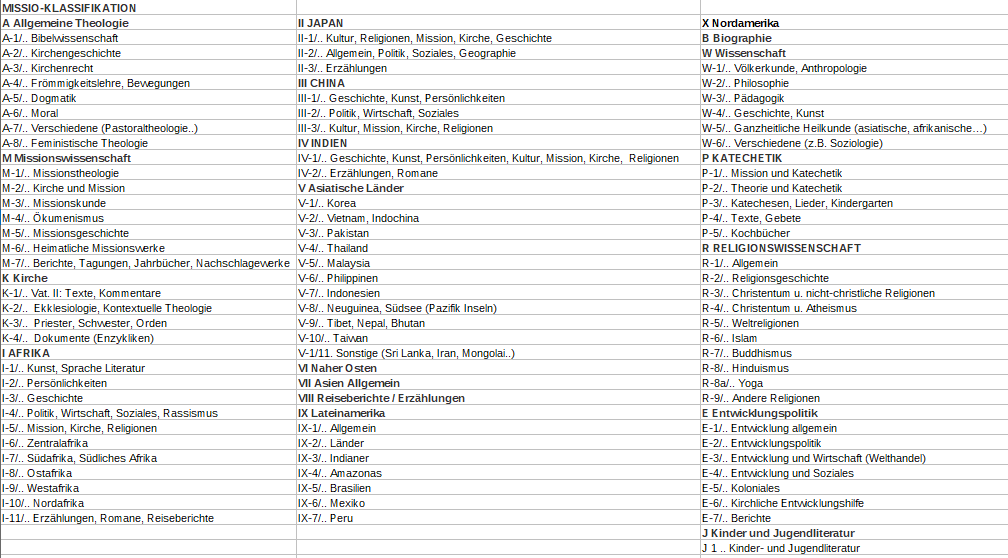
\includegraphics{img/img1.PNG}
\end{figure}

Vorbemerkung der LIBREAS-Redaktion:

Das nachfolgende Interview entstand im Rahmen der zwei Projektseminare,
die LIBREAS am Institut für Bibliotheks- und Informationswissenschaft
der Humboldt-Universität der Berlin im Wintersemester 2020/2021
beziehungsweise im Sommersemester anbot. Es zeigt die Möglichkeiten und
auch die Grenzen einer integrativen und interkulturellen Produktion von
Inhalten. Auf der Seite der Möglichkeiten steht zunächst das
außergewöhnliche Aktivierungspotential, dass das Thema Dekolonisierung
bei Studierenden des Faches besitzt. Das Engagement überraschte uns sehr
und ebenso, dass fast alle, die sich jeweils eingeschrieben hatten, auch
-- obwohl sie, wie das an Universitäten üblich ist, hätten jederseits
problemlos abbrechen können -- bis zum Ende dabei blieben. Angesichts
der besonderen Umstände des pandemiebedingten Digitalsemesters ist das
nicht selbstverständlich. Eine glückliche Fügung ermöglichte zudem einen
Austausch, der, wie wir feststellen, deutlich zu selten möglich ist.
Gerade aber, wenn wir im Zusammenhang mit Fragen der Dekolonisierung die
eurozentrische Ausrichtung des Bibliothekswesens reflektieren, benötigen
wir eigentlich die Sichtweisen, die dezidiert nicht westlich geprägt
sind. Mit Valentina de Toledo hatten wir eine Teilnehmerin, die an
dieser Stelle, wenn man so will, vermitteln konnte. Als gebürtige
Brasilianerin, die in Berlin lebt, hat sie einen Verständnishorizont,
aus dem wir an sich viel lernen können. Angeregt durch die
Fragestellungen des Seminars entschied sie sich als Seminarprojekt ein
Interview mit einer der herausragenden Aktivistinnen einer Bewegung der
\enquote{bibliotecárias/os negras/os e antirracistas} zu führen.
Franciéle Carneiro Garcês da Silva hat Bibliothekswissenschaft am
Instituto Brasileiro de Informação em Ciência e Tecnologia (IBICT) in
Rio de Janeiro und an der Universidade do Estado de Santa Catarina
(UDESC) studiert und wirkt in diversen Initiativen dessen mit, was wir
in Deutschland vielleicht als \enquote{kritische
Bibliothekswissenschaft} bezeichnen würden. Sie koordiniert die
\enquote{Grupo de Estudos Mulheres Negras na Biblioteconomia e Ciência},
welche sich mit der Rolle und den Perspektiven Schwarzer Frauen im
Bibliothekswesen und in der Bibliothekswissenschaft beschäftig. Aus der
Forschungsarbeit dieser Gruppe entstanden zahlreiche Publikationen, die
unter \url{https://www.nyota.com.br/livros} verzeichnet sind und jeweils
auch als PDF heruntergeladen werden können.

Wir freuen uns außerordentlich, ihren Blick auf Whiteness\footnote{Wir
  übersetzen den Begriff Whiteness in diesem Zusammenhang nicht. Zwar
  findet sich im deutschen Diskurs auch die Variante \emph{weiß}-sein
  oder weißsein, im Sinne zum Beispiel von ``kritschen
  \emph{weiß}-seinsforschung. Aber wir sehen eine erhebliche Differenz
  in der Bedeutungsgeschichte von Whiteness und dem Attribut
  \emph{weiß}, die im vorliegenden Rahmen nicht zureichend gespiegelt
  werden kann. Daher entscheiden wir uns für die etabliertere englische
  Bezeichnungen. (Anmerkung der Redaktion)} und Rassismus in der
Bibliotheks- und Informationswissenschaft abbilden zu können. Allerdings
offenbaren sich an diesem Punkt auch die Grenzen. Denn wie sich zeigte,
ist eine geradlinige Übersetzung des ursprünglich in brasilianischem
Portugiesisch geführten Interviews deutlich komplizierter als wir und
als die Seminarteilnehmer*innen aus dem Sommersemester, die dies als
Seminarprojekt übernahmen, zunächst dachten. Inklusive Sprache an sich
ist eine Übersetzungsherausforderung. Die Übertragung des Gesprochenen
in eine schriftsprachliche Form eine zweite. Und schließlich gibt es den
kulturellen Hintergrund, der nicht nur die Besonderheiten der
brasilianischen Gesellschaft sondern in diesem Fall auch die des
brasilianischen Hochschulwesens betrifft. Bei den redaktionellen
Bearbeitungen stellten sich häufig Anschlussfragen, die wir leider nicht
umfassend nachverfolgen konnten. Die deutsche Interviewfassung
entspricht daher dem, was uns unter unseren Produktionsbedingungen
bestmöglich war. Dies gilt gleichermaßen für die englische Übersetzung.
Um Klarheit und Lesbarkeit herzustellen, wurden diese Fassungen gekürzt.
Parallel publizieren wir die Transkriptionsfassung im brasilianischen
Portugiesisch. Sollte es zu Übertragungsfehlern gekommen sein, bitten
wir um Nachsicht und Hinweise.

\textbf{Valentina de Toledo (VT): Vielen Dank für deine Zeit und
Bereitschaft, unsere Fragen zu beantworten. Die Bibliothek ist ein Ort,
an dem viele Welten aufeinandertreffen. Sie ist aber auch ein Ort, an
dem sich Muster der Gesellschaft wiederholen, darunter Rassismus und
andere Formen der Diskriminierung. Wir würden gern mehr über deine Sicht
als Erkenntnistheoretikerin und Doktorandin der Informationswissenschaft
auf die Auswirkungen der so genannten Whiteness in diesem Bereich und
insbesondere im brasilianischen Bibliothekswesen erfahren.}

\textbf{In dem Buch \enquote{Epistemologias Latino-Americanas}
(Lateinamerikanische Epistemologien) \linebreak fragst du: \enquote{Rassismus ist ein
\emph{weißes} Thema, warum sollten sich nur Schwarze in ihrer Lehre und
beruflichen Praxis damit befassen?} Ich würde dich bitten, zunächst
einmal darüber zu sprechen, was Whiteness für dich bedeutet?}

Franciéle Carneiro Garcês da Silva (FS): {[}Der Autor und
Journalist\footnote{\url{https://en.wikipedia.org/wiki/Ta-Nehisi_Coates}
  (Anmerkung der Redaktion)}{]} Ta-Nehisi Coates formulierte es so:
\enquote{Race ist das Kind des Rassismus, nicht seine Mutter.} Davon ausgehend
spreche ich in meinem Buch davon, dass Whiteness \enquote{die Mutter des
Rassismus} ist. Das Konzept der Race\footnote{Wir verwenden in der
  Übersetzung vorwiegend den Ausdruck Race, da das deutsche Wort
  \enquote{Rasse} semantisch nicht mit der Wortbedeutung identisch ist,
  die hier gemeint ist. Im vorliegenden Fall geht es bei Race um eine
  Kategorisierung von Menschen aufgrund sozialer und äußerer Merkmale.
  Dem deutschen Ausdruck \enquote{Rasse} fehlt unserer Ansicht nach im
  Unterschied zu \enquote{Rassismus} zu großen Teilen wenigstens die
  soziale Perspektive, was erfahrungsgemäß im Diskurs oft zu
  Fehldeutungen führt. Wo uns eine Verwendung der Bezeichnung
  \enquote{Rasse} als für die Aussage relevant erschien, wird dies durch
  Anführungszeichen hervorgehoben. (Anmerkung der Redaktion)} wurde
benutzt, um Menschen zu klassifizieren. Dahinter steht eine
Hierarchisierung in \enquote{überlegene und minderwertige Rassen}. Dies hat den
Zweck, zu trennen und zu dominieren. Whiteness bezieht sich auf die
Identität, die in Entsprechung zu lokalen und globalen Einflüssen
entsteht und rekonstruiert wird. Whiteness als Praxis etablierte sich
historisch in dem Moment, in dem europäische und amerikanische
\emph{weiße} Männer das Konzept der Race heranzogen, um andere Menschen
kolonisieren, dominieren und versklaven zu können. Dies geschah, wie im
Fall der afrikanischen Bevölkerungen, auch im Rückgriff auf
pseudowissenschaftliche und religiöse Vorstellungen der jeweiligen Zeit,
was, zusätzlich zur geschaffenen Machtstruktur, eine Legitimation
sicherte.

Wenn ich sage, dass Whiteness die Mutter des Rassismus ist, dann
schließe ich keinesfalls aus, dass es schon vor der Einführung des
Konzepts menschlicher \enquote{Rassen} Vorurteile mit ähnlichen
Wirkungen gab. Doch seit das Konzept der Race zur Anwendung kommt, sind
es die damit verbundenen äußeren und sozialen Merkmale, die zur
Hierarchisierung und Klassifizierung von Menschen mit Betonung der
danach nicht-\emph{weißen} Gruppen dient. Die über rassische Merkmale
bestimmte \emph{weiße} Identität wird seitdem so behandelt, als gäbe es
überlegene und unterlegene \enquote{Rassen}. Dieses Rassenprivileg
findet sich auch heute in sämtlichen Teilen der brasilianischen
Gesellschaft.

Wenn ich also betone, dass Rassismus ein \emph{weißes} Problem ist, dann
spreche ich von einem Konzept oder Modell, in dem Whiteness historisch
etwas verankerte, das bis heute in der brasilianischen Gesellschaft als
Instrument zur Unterdrückung nicht-\emph{weißer} Menschen zum Einsatz
kommt. Im Fall Brasiliens sind dies die Indigenen, Schwarze Menschen
afrikanischer Herkunft und auch die LGBTQIA-Bevölkerung,\footnote{Akronym
  für die englischen Bezeichnungen: \enquote{Lesbian, Gay, Bisexual,
  Transsexual/-gender, Queer, Intersexual und Asexual}.} die nicht der
cis-heterosexuellen Hegemonie entspricht. Dieses von der Elite
propagierte Herrschaftselement einer Überlegenheit
\enquote{\emph{weißer} Merkmale} wirkt nicht nur im Bereich der Race,
sondern auch in Bezug auf Geschlecht, Klasse und Sexualität, außerdem
können mehrere dieser Bereiche ein und dieselbe Person betreffen. Dann
wird von Intersektionalität gesprochen.

\textbf{VT: Wie zeigt sich dies in der brasilianischen Gesellschaft?}

FS: In Brasilien sehen sich \emph{weiß} gelesene Personen als Träger
einer vermeintlichen Normalität. Sie sehen und setzen sich selbst als
den zu erreichenden Standard. \emph{Weiß} zu sein, ist in ihren Augen
das Normale. Diejenigen, die von diesen \emph{weiß} gesetzten Normen
abweichen, streben danach, einen sozialen Status zu erreichen und in der
Gesellschaft akzeptiert zu werden, indem sie sich dem anzunähern
versuchen. Dies geschieht teils äußerlich, indem man versucht die
Gesichtszüge aufzuhellen oder die Haare glättet, um einer \emph{weißen}
Ästhetik zu entsprechen. Teils über die Übernahme der Diskurse und
Deutungsmuster der Meritokratie\footnote{Vorstellung, dass Positionen in
  der Gesellschaft (Status, ökonomische Stellung et cetera) alleine
  durch die Leistung einer Person bestimmt ist. (Anmerkung der
  Redaktion)} der auf dem Differenzierungsmerkmal \enquote{Race}
basierenden brasilianischen Gesellschaft. Oder durch Veränderungen des
Verhaltens, einer Abkehr von kulturellen und habituellen Merkmalen
Schwarzer oder indigener Kulturen.

Brasilien war sehr lange eine Kolonie und das in dieser Geschichte
verinnerlichte koloniale Denken wirkt bis heute. Daher werden
rassistische Einstellungen oft nicht hinterfragt, sondern gelten als
gerechtfertigt. Für die betroffenen Teile der Bevölkerung ist dies ein
grundsätzliches Hindernis. Die Politik verfolgt weiterhin das Ziel,
\emph{weiße} Migrant*innen nach Brasilien zu holen und somit Brasilien
selbst zunehmend \emph{weiß} zu machen. Der Diskurs des \emph{weißen}
Brasiliens wird exportiert. Als Idealbild einer brasilianischen Frau
gilt Giselle Bündchen,\footnote{Brasilianisches Modell
  \url{https://de.wikipedia.org/wiki/Gisele_B\%C3\%BCndchen} (Anmerkung
  der Redaktion)} die aus einer Region Brasiliens stammt, die vorwiegend
durch europäische Einwander*innen geprägt ist. Viele denken nun also,
dass Frauen aus Rio Grande do Sul wie Giselle Bündchen aussehen.
Außerdem verlieren sich mit dem Whitening der Gesellschaft andere
Traditionen und Wissensformen, die für die afrikanische und
afrobrasilianische Kulturen prägend waren, wie zum Beispiel Capoeira
oder Samba. Andere Elemente afrikanischer Herkunft wurden historisch
über Verbote verdrängt. Dazu zählen Formen afro-brasilianischer
Religiosität wie Candomblé und Batuque.\footnote{Afrobrasilianische
  Religionen \url{https://en.wikipedia.org/wiki/Candombl\%C3\%A9}
  \url{https://de.wikipedia.org/wiki/Batuque} (Anmerkung der Redaktion)}Diese
wurden während und nach der Zeit der Sklaverei unterdrückt. Auch heute
gibt es Angriffe von Evangelikalen auf Umbanda- und
Candomblé-Terreiros.\footnote{Afrobrasilianische Religionen
  \url{https://de.wikipedia.org/wiki/Umbanda}
  \url{https://de.wikipedia.org/wiki/Candombl\%C3\%A9} (Anmerkung der
  Redaktion)} Ziel solcher Attacken ist seit je das Kappen der
kulturellen Wurzeln von Menschen afrikanischer und afro-brasilianischer
Herkunft, um ihr Denken und ihre Körper dominieren und kolonisieren zu
können.

Man muss dabei berücksichtigen, dass \emph{weiß} in Brasilien etwas
anders ist als in Europa oder den USA. Auch innerhalb Brasiliens gibt es
Unterschiede. Eine \emph{weiße} Person wird im Süden Brasiliens anders
gelesen als im Nordosten. Neben äußerlichen Merkmalen gibt es weitere
Aspekte, die dazu führen, dass eine Person innerhalb unserer
rassifizierten Gesellschaft als mehr oder weniger \emph{weiß}
wahrgenommen wird. Die Professor*innen Lourenço Cardoso und Liv Sovik
sprechen viel darüber, was es bedeutet, in Brasilien \emph{weiß} zu sein
und was der Unterschied zwischen diesen Ausprägungen der Whiteness ist.

\textbf{VT: Wie ist es im universitären Kontext?}

FS: Ein aktuelles Beispiel für den Ausdruck der Whiteness in der
akademischen Welt Brasiliens ist das Ausnutzen von Quoten, die für
nicht-\emph{weiße} Gruppen eingeführt wurden. Es passiert, dass
\emph{weiße} Menschen Quoten missbräuchlich für sich reklamieren, die
eigentlich zum Beispiel für Nachfahren der indigenen Bevölkerung oder
Quilombolas\footnote{Während der Sklaverei in Brasilien dieser
  entflohene Menschen \url{https://de.wikipedia.org/wiki/Quilombo}
  (Anmerkung der Redaktion)} etabliert wurden. Auch hier nutzen sie
abermals das Privileg ihrer Whiteness aus. Dass sie zu einer Gruppe
gehören, die ohnehin historisch und gesellschaftlich begünstigt ist,
blenden sie ebenso aus, wie 300 Jahre Versklavung Schwarzer Menschen in
Brasilien. Schwarze Menschen erhielten bis heute keine Kompensation für
die Jahrhunderte der Sklaverei, weder materiell noch immateriell.
Zugleich wird ihnen der Zugang zu Bildung erschwert.

\textbf{VT: Warum haben viel \emph{weiße} Menschen ein Problem damit,
sich als privilegierte Gruppe zu sehen?}

FS: Oft wird dies mit einem \emph{Mythos der Egalität} beiseite
geschoben. Dieser besagt, dass in unserer Demokratie ja formal alle
Menschen unabhängig ihrer Herkunft gleich sind. Dazu kommt einer
verinnerlichte Meritokratie. Wem der soziale Aufstieg nicht gelingt,
die*der scheitern nur wegen fehlenden Bemühens. Hinter diesen beiden
Punkten werden die historisch in die brasilianische Gesellschaft
eingeschriebenen Benachteiligungen ausgeblendet.

Man kann durchaus fragen, warum man trotz der Quoten so wenige Schwarze
Menschen an den Universitäten findet und wo eigentlich die Schwarzen
Professor*innen sind, die formal da sein sollten? Wenn alle die gleichen
Chancen und Fähigkeiten haben, müssten sich doch alle gleichermaßen in
den Bereichen der Macht finden.

Der \emph{Mythos der Bestenauslese} ist ein künstliches Instrument, um
die brasilianische Gesellschaft formell zu nivellieren, die Verhältnisse
aber zu bewahren. Tatsächlich sind die Chancen für Schwarze Menschen
ganz anders als die \emph{weißer} Menschen.

Ein weiterer Effekt des \emph{Mythos' der Meritokratie} ist, dass die
\emph{weißen} Menschen ihren Wohlstand und ihre soziale Stellung allein
ihrer harten Arbeit zuschreiben. Aber wie häufig sieht man, dass bei der
Besetzung von Führungspositionen Netzwerke entscheiden?

Historisch waren es tatsächlich die Sklaven, die den Wohlstand
erarbeitet haben. Die \emph{weißen} Menschen haben sich den Wert dieser
Arbeit unrechtmäßig angeeignet. In der Logik der Meritokratie würde er
ihnen also gar nicht zustehen.

Dazu kommt der konkrete Rassismus, der \emph{weißen} Menschen positive
Eigenschaften zuschreibt, Schwarzen und indigenen Menschen dagegen
vorwiegend negative. Die Vorstellungen überlegener und minderwertiger
Rassen wirken immer noch. Rassistisch denkende Menschen gehen davon aus,
dass sie natürlicherweise überlegen sind. Ob bewusst oder unbewusst
entmenschlichen sie damit andere. Ohne dass sie es wahrnehmen, werden
ihre entsprechenden Handlungen von Betroffenen als übergriffig und
gewaltsam empfunden.

Auch werden formal bestehende Rechte oft schlicht verweigert. Warum sind
Schwarze Menschen bis heute in höchstem Maße von Ungleichheit und
sozialer, wirtschaftlicher und schulischer Benachteiligung betroffen?
Weil nach der Abschaffung der Sklaverei den Schwarzen -- neben den
Folgen der Sklaverei -- ihre Rechte auch von staatlicher Seite
verweigert wurden. Die öffentliche Politik zeigte kein Interesse an
ihrer Bildung, ihrer Entwicklung und ihrem sozialen Aufstieg. Der
Anthropologe Kabengele Munanga\footnote{\url{https://pt.wikipedia.org/wiki/Kabengele_Munanga}
  (Anmerkung der Redaktion)} vertritt die These, dass der Rassismus in
Brasilien deshalb wirksam ist, weil das, was eine Person sagt, nicht
immer das ist, was sie meint. Für mich ist es immer dann Rassismus, wenn
eine Schwarze Person durch etwas, das gesagt oder getan wird,
eingeschränkt oder verletzt wird. Dies kann aber nicht in jedem Fall so
offen benannt werden.

\textbf{VT: Wird Rassismus also ausschließlich von \emph{weißen}
Menschen ausgeübt?}

FS: \emph{Weiße} Menschen reproduzieren Rassismus durch ihre Wahrnehmung
und ihr Handeln. Das heißt nicht, dass Schwarze Menschen nicht -- und
das ist das richtige Wort -- Rassismus reproduzieren können. Denn in
einer rassistischen Gesellschaft lernen und verinnerlichen sie genau
das. Wenn es keine Aufklärung und keinen Diskurs gibt, der freilegt, wie
Race und Rassismus in unserer Gesellschaft wirken, werden sie den
Diskurs der Unterdrückenden weiter reproduzieren. Schwarze Menschen in
Brasilien haben oft keinen Zugang zu ihrer eigenen Geschichte, weil die
entsprechenden Dokumente und Aufzeichnungen weitgehend vernichtet
wurden, und zwar aus Angst, dass künftige Generationen Wiedergutmachung
verlangen würden. Der \emph{Mythos der Gleichheit} bewirkt, dass sie oft
nicht sehen, welchen Einfluss Rassismus auf ihr Leben hat. Der
\emph{Mythos der Meritokratie} bewirkt häufig, dass ihre begrenzten
Aufstiegschancen auf mangelndes individuelles Bemühen zurückgeführt
werden.

Eine wichtige Sache, die man verstehen muss, und die auch Professorin
Lia Vainer Schucman betonte, ist, dass man, selbst wenn man eine
ökonomisch arme \emph{weiße} Person ist, immer das \enquote{Privileg der
Hautfarbe} haben wird. Dieses Privileg strukturiert die Beziehungen und
steuert den Zugriff auf Chancen, Güter und Status innerhalb der
brasilianischen Gesellschaft.

\textbf{VT: Wie zeigt sich dieses Privileg?}

FS: Es bezieht sich auf alle gesellschaftlichen Vorteil der Whiteness.
Das kann zum Beispiel sein, dass man auch als arme \emph{weiße} Person
bestimmte Räume betreten kann, ohne vom Sicherheitsdienst hinausgeworfen
zu werden. Oder, dass man als epistemische Autorität zu einem bestimmten
Thema angesehen wird, auch ohne es tief studiert zu haben. Es reicht
aus, dass man sich äußert. Vor nicht allzu langer Zeit haben drei
\emph{weiße} Personen einen Artikel über Affirmative-Action-Themen
geschrieben, obwohl sie nicht auf dem Gebiet arbeiten. Entsprechend
standen einige absurde Dinge darin. Er wurde trotzdem veröffentlicht.

Zugleich werden wissenschaftlich fundierte Artikel von Schwarzen zu
solchen Themen mit der Begründung, sie seien politisch, militant oder
radikal, abgelehnt.

Dies geschieht, weil die Wissenschaft selbst in Bezug auf ihren
Rassismus einen blinden Fleck hat. Dass wir in der brasilianischen
Bibliothekswissenschaft so wenige Artikel oder Bücher zum Thema haben,
ist kein Wunder. Und von den wenigen Publikationen zum Thema stammen
viele von \emph{weißen} Autor*innen, die über Schwarze schreiben. Der
Faktor Race wird immer einen Einfluss haben, wenn Schwarze Menschen über
ihre Erfahrungen und ihre Sicht auf die Geschichte schreiben, wenn sie
ihre kritische Perspektive und wissenschaftliche Bewertung einbringen
und sie dabei immer mit den Mythen der Egalität, der Meritokratie und
immer Effekten von Whiteness und Rassismus konfrontiert werden.

\emph{Weiße} Menschen werden folglich immer ablehnend reagieren,
entweder, weil sie nichts von dem Thema verstehen, oder weil sie diese
Debatten für unnötig halten, da sie sich in einer Gesellschaft befinden,
die aus ihrer Sicht fair und für alle gleich ist. Diese Ausgrenzung von
Perspektiven, Deutungen und Wissen ist ein Epistemizid. Dieses Konzept,
das von Boaventura de Sousa Santos und Sueli Carneiro breit diskutiert
wird, beschreibt eine Auslöschung des von Schwarzen und unterdrückten
Menschen produzierten Wissens. Der Hauptgrund dafür ist, dass es eine
Gegenerzählung darstellt zu dem vom hegemonialen Kontext produzierten.
So überrascht es nicht, wenn Professor*innen sagen, sie hätten noch nie
etwas über diese Themen gelesen, oder, dass ein Buch, das 2018 erschien,
das Erste zu dieser Diskussion sei, obwohl das Thema in der Bibliotheks-
und Informationswissenschaft tatsächlich schon lange diskutiert wird.

\textbf{VT: Und wie beeinflusst Whiteness das Bibliothekswesen und die
Bibliotheks- und Informationswissenschaft (LIS)?}

FS: Im Bibliothekswesen erfolgt ihr Einfluss auf verschiedene Weise. Da
ist zunächst der Glaube an die Existenz verschiedener \enquote{Rassen},
wobei einige als Inhaber und Produzenten von Wissen angesehen werden und
andere nicht. Es ist, als ob diese Populationen kein Wissen hätten, kein
Wissen produzierten, nicht epistemologisch über ihre Wissensbereiche und
ihre sozialen Realitäten, über das Sein und ihr Dasein in der Welt
reflektierten. So wird ein normatives Modell von Wissenschaft
geschaffen, das den im Globalen Norden etablierten Standards folgt.

Zweitens ist das Bibliothekswesen in Brasilien vom europäischen und
amerikanischen Bibliothekswesen geprägt. Damit wird das etabliert, was
ich als \emph{White Librarianship} bezeichnen würde. Die theoretischen
Grundlagen und Bezüge sind ebenso stark eurozentristisch wie die
Perspektive auf die Wissenschaft und das wissenschaftliche Arbeiten. Das
dekoloniale Wissen sowie das Wissen von Menschen, die sich am Rande
dieser Gesellschaft befinden, bleibt außer Acht.

Nimmt man diese beiden Einflüsse zusammen, haben wir einen Epistemizid.
Wissen, das innerhalb der Universität als minderwertig angesehen wird,
ist de facto inexistent. Menschen, die in ihren Studien- oder
Abschlussarbeiten über Race und Rassismus im Bibliothekswesen schreiben
wollen, werden mit dem Argument davon abgehalten, dass diese
Diskussionen kein Forschungsfeld der Bibliothekswissenschaft ist.

Race und die damit verbundenen Fragen werden unsichtbar gemacht. So
kommt es dazu, dass Dozent*innen, indem sie europäischen Theorien und
Modellen folgen, nicht in der Lage sind, die Situation und
Lebenskontexte der Studierenden zu verstehen. Schwarze und indigene
Studierende müssen sich der gleichen Messlatte fügen wie \emph{weiße}.
Es wird so getan, als hätten alle die gleichen Voraussetzungen, was in
Brasilien nicht gegeben ist.

\textbf{VT: Whiteness wirkt also auch in der Lehre?}

FS: Die benannten Mythen prägen auch das Bildungswesen. Ein*e
Professor*in, der*die denkt, dass jede*r an der Universität aus einer
Situation kommt, in der es üblich ist, auf Englisch studieren zu können,
die Publikationsformen kennt und weiß, wie man was schreibt, reflektiert
nicht darüber, wie dies von vornherein Menschen diskriminiert, die nicht
mit diesem Wissen an die Universität kommen. Es gibt auch
Professor*innen, die Studierende wegen dieser fehlenden Vorkenntnisse
schlechter benoten. Schwarze Menschen sind aber nicht immer auf die
Bedingungen und Mechanismen der Wissenschaft vorbereitet, wenn sie an
die Universität kommen. Es gibt häufig ein Bildungsdefizit, weil sie
meistens von öffentlichen Schulen kommen. Schaffen sie es auf die
Universität, werden sie dort in vielen Fällen mit finanziellen,
pädagogischen und linguistischen Überforderungen konfrontiert. Es gibt
zum Beispiel keine vorbereitende Vermittlung von Informationskompetenz,
sodass wir an der Universität ankommen und bereits wissen müssen, welche
Parameter es zu erfüllen gilt und wie wir uns in diesem Raum behaupten
können, der ein historisch \emph{weißer}, eurozentrierter,
euroamerikanisierter Raum ist. Ganz zu schweigen von den rassistischen
Witzen von Professor*innen, die ich in meinem Kurs oft erlebt habe,
einem, wie der Autor Adilson Moreira nennt, \enquote{Recreational
Racism}.

\textbf{VT: Was ist das?}

FS: Adilson Moreira zeigt in seinem Buch \enquote{Recreational Racism}, dass
Recreational Racism auf rassistischen Witzen basiert, deren Pointe
darauf aufbaut, dass von Schwarzen immer erwartet wird, dass sie etwas
falsch machen. Das eine reine Erfindung, die einen rassisch-ethnischen
Aspekt enthält, obwohl tatsächlich jede Person Fehler machen kann,
unabhängig davon, ob sie Schwarz ist oder nicht.

\textbf{VT: Auf welche Schwierigkeiten stoßen Schwarze Menschen in der
Universität?}

FS: Die Hürden liegen sowohl in den Teilhabemöglichkeiten zum Beispiel
bei Forschungsprojekten, als auch im Inhaltlichen. So werden in
postgraduierten Projekten innerhalb der Programme bestimmten Themen
nicht genehmigt. Dabei ist es oft so, dass diese subjektiven
Entscheidungen von den Entscheider*innen oft gar nicht als rassistisch
wahrgenommen werden. Das kann unbewusst erfolgen, denn in diesen Fällen
fehlt meistens ein Verständnis dafür, dass die Gesellschaft rassistisch
ist.

Erst seit den 2000er-Jahren gab es bei der ENACIB\footnote{Encontro
  Nacional de Pesquisa em Ciência da Informação -- die zentrale
  informationswissenschaftliche Konferenz Brasiliens.} einen
bibliothekswissenschaftlichen Beitrag zum Thema \enquote{Whiteness in Teaching
Practices in Librarianship and Information Science}\footnote{\url{https://brapci.inf.br/index.php/res/v/102318}},
geschrieben von mir, Gustavo Saldanha und Daniela Pizarro. Das ist
erstaunlich, da es \emph{Critical Whiteness Studies} im Bibliothekswesen
auch schon länger gibt. Die afrokanadische Bibliothekarin und Forscherin
Jody Nyasha Warner war eine der Ersten, die sich mit dem Thema
auseinandersetzte.\footnote{siehe unter anderem Jody Nyasha Warner
  (2005): Africa in Canadian Academic Libraries: A Continent's Voices Go
  Missing. In: Social Justice, Vol. 32, No.~4 (102), S. 180--191.
  \url{http://www.jstor.org/stable/29768343} (Anmerkung der Redaktion)}
Erwähnenswert sind auch die Arbeiten der Lehrerin und Bibliothekarin
Isabel Espinal zur Whiteness in Bibliotheks- und
Informationswissenschaft. Dirnéle Garcez und ich haben über sie in
unserem Buch \enquote{Bibliotecári@s Negr@s}\footnote{Franciéle Carneiro Garcês
  da Silva, Graziela dos Santos Lima (Hrsg.): Bibliotecári@s Negr@s:
  ação, pesquisa e atuação política. Florianópolis, SC: Associação
  Catarinense de Bibliotecários, 2018.

  bzw.

  Franciéle Carneiro Garcês da Silva, Dirnéle Carneiro Garcês: SABEL
  ESPINAL E SUAS

  CONTRIBUIÇÕES PARA BIBLIOTECONOMIA E CIÊNCIA DA INFORMAÇÃO (BCI). In:

  Franciéle Carneiro Garcês da Silva; Nathália Lima Romeiro (Hrsg.): O
  protagonismo da mulher na biblioteconomia e ciência da informação:
  celebrando a contribuição intelectual e profissional de mulheres
  latinoamericanas. Florianópolis, SC: Rocha Gráfica e Editora, 2020.
  (Selo Nyota) S.130--151 (Anmerkung der Redaktion)} geschrieben.

\textbf{VT: Es ist bemerkenswert, dass Schwarze Menschen die höchste
Quote von Studienabbrüchen in der Bibliothekswissenschaft haben (71,7
\%). Siehst Du Whiteness als ursächlichen Faktor?}

FS: Sie brechen oft ab, weil sie sich in den Curricula nicht
wiedererkennen. Sie brechen aber auch ab, weil sie es sich oft nicht
leisten können. Auch öffentliche Universitäten kosten Geld. Dazu kommen
Umzugskosten, Reisekosten, Miete, Essen und so weiter. Die Unterstützung
der Hochschulen ist gering. Hilfsprogramme gibt es kaum oder sie sind
Schwarzen Studierenden kaum bekannt. Generell ist es so, dass das
Regelstudium nur für Menschen passt, die sich tagsüber freinehmen
können, also privilegiert sind. Viele Schwarze Menschen müssen arbeiten
und ihre Familie versorgen, können also nur Abendkurse wählen.

Hinzu kommen rassistische Effekte: Den Schwarzen Menschen wird
vermittelt, dass dieser \linebreak Raum, also die Hochschule, nicht für sie ist.
Sie fühlen sich isoliert, teils verfolgt von Lehrer*innen, von
Kolleg*innen oder von Erfahrungen mit institutionellem Rassismus. Wo sie
nicht offen aufgenommen werden, halten sie auch nicht durch.

\textbf{VT: Setzt Du in der Lehre auf Material von Schwarzen oder
indigenen Brasilianer*innen oder eher von \emph{weißen}
Brasilianer*innen oder Menschen aus dem Globalen Norden?}

FS: Die Autor*innen in unserem Bereich sind meist \emph{weiß}. Schauen
wir zum Beispiel auf die epistemologischen und historischen Studien der
Bibliothekswissenschaft, finden wir nahezu ausschließlich \emph{weiße}
Stimmen. Zu nennen wären: Gustavo Saldanha, César Karpinski, Solange
Mostafa, Carlos Alberto Ávila Araújo, Oswaldo Almeida Júnior, Henriette
Gomes und andere. Es gibt aber einige Schwarze Autor*innen, auf die wir
uns beziehen können, zum Beispiel Maria Aparecida Moura, Mirian de
Aquino, Ana Cláudia Borges, Ana Paula Menezes, Leyde Klébia Rodrigues,
Francilene Cardoso. Sie leisten ihren Anteil am
bibliothekswissenschaftlichen Wissen, werden aber nicht immer in der
Lehre der Bibliothekswissenschaft in Brasilien vermittelt. In den
Büchern von Schwarzen zum Bibliothekswesen kommen sie natürlich vor.
\enquote{Bibliotecári@s Negr@s} und \enquote{O Negro na Biblioteca} sind zwei Titel, die
sich mit bibliothekswissenschaftlichen Fragen aus dieser Perspektive
befassen. Im Gesamtspektrum des wissenschaftlichen Publizierens
dominieren jedoch \emph{weiße} Autor*innen und werden auch häufiger
zitiert.

Man findet aber auch in der Bibliothekswissenschaft \emph{weiße}
Menschen, die einen kritischen und
geisteswissenschaftlichen-differenzierenden Blick einbringen. Ich möchte
dahingehend Francisco das Chagas Júnior und Daniella Pizarro
herausheben. Beide sind wichtige Referenzen für ethische Aspekte des
Berufs und des Bibliothekswesens. Sie kritisieren die technizistische
Orientierung, die für eine mehr geisteswissenschaftlichen Perspektive
ein Nachteil ist. Weiterhin wäre Jacqueline Cabral, eine Archivarin,
welche archiv-theoretische Fragen von Gender und Sexualität untersucht,
zu nennen.

\textbf{VT: Was meinst Du in diesem Fall mit Technizismus?}

FS: Wir sehen einen sehr starken Trend in der Bibliothekswissenschaft
zur Ausrichtung auf die Informations- und Kommunikationstechnologien.
Geisteswissenschaftlichere Fragestellungen werden dagegen
zurückgestellt.

Eine Debatte darüber wurde von Maria Aparecida Moura, Rubens Alves da
Silva und Fabrício Nascimento angeregt. Diese Professor*innen sind sehr
wichtig, denn nur sie können den Diskurs innerhalb der Hochschulen
wirklich anstoßen. Schwarze Menschen haben als traditionell
benachteiligte Gruppen wenig Wirkungsmöglichkeiten in diesen Räumen.

\textbf{VT: Sind denn die geisteswissenschaftlichen Sichtweisen auf die
Bibliotheks- und Informationswissenschaft weithin akzeptiert?}

FS: Aus meiner Sicht sind sie es nicht. Ich merke das an dem Widerstand,
den es gibt, wenn man ein unbequemes Thema wie Whiteness oder
struktureller Rassismus einbringt. Die Gruppe, die von institutionellen
oder auch sprachlichen Rassismen profitiert, setzt nach wie vor ihre
Dominanz ein, um Schwarze, indigene, LGBTQIA- und Menschen mit
Behinderungen aus den Bereichen der Deutungshoheit auszuschließen und
deren Diskurse, teils auch ihre Existenz in akademischen Räumen
unsichtbar zu machen. Die technizistische Ausrichtung des
Bibliothekswesen fördert dies, denn es erleichtert die Vorspiegelung von
Neutralität.

\textbf{VT: Inwiefern ist die Bibliothek für Dich ein \enquote{Machtraum} für
die Propagierung und Durchsetzung solcher Mechanismen?}

FS: Man muss sich nur nur ansehen, wie die Vermittlung von Kinderbüchern
zum Beispiel Aschenputtel und Disney-Klassiker in den Mittelpunkt rückt,
afrikanische, afro-brasilianische oder auch indigene Geschichten aber
kaum abbildet. Ebenso wie LGBTQIA-Literatur finden sie sich kaum in
Bibliotheken. Auch in der Ausbildung kommen diese anderen Perspektiven
nicht vor. Für mich zeigt sich darin elementar die Förderung eines
Diskurses zugunsten von Whiteness, als eines Privilegs und der
Aufrechterhaltung dieses Privilegs, in dem \emph{weiße} Maßstäbe als
allgemeiner Standard gesetzt werden.

\textbf{VT: Wie gehst Du mit dieser Tatsache um?}

FS: Als Information Professional muss ich mich kritisch und politisch
dazu positionieren. Ich muss verstehen, das jedes Element der Ausbildung
und der Curricula politisch ist. Sobald ich mich für einen bestimmten
Diskurs entscheide, der andere unsichtbar macht, ist es eine politische
Entscheidung.

Da es immer politisch ist, muss ich mich entscheiden. Ich kann einen
Diskurs wählen, der antirassistisch und dekolonial ist. Oder ich kann
einen Diskurs wählen, der die Anforderungen des Kapitalismus bedient,
einen hegemonialen Diskurs, der die Neutralität der Wissenschaft
behauptet, eine Literatur die \enquote{eine einzige Geschichte} fördert
, in der, wie Chimammanda Adichie sagt, nur \emph{weiße} Männer als
Klassiker betrachtet werden, Frauen kaum gelesen werden und Schwarze
Frauen nicht einmal bekannt sind.

Wenn wir die Universität so wahrnehmen und hinnehmen, wird sich nichts
ändern. Wir werden immer eine bestimmte Vorstellung von Identität
fördern und das Privileg der Whiteness durch das, was wir lesen, tun und
sagen, aufrecht erhalten. Eine Umgestaltung der Universität und der
Ausbildung ist enorm komplex und schwierig. Denn sobald man Teil der
Universität ist, ist man am Ort der Elite.

In den Grundkursen werden Leute, die nicht selbst mit Rassismus
konfrontiert sind, nicht verstehen, warum das Thema überhaupt diskutiert
wird und Teil der Berufsausbildung sein sollte. Ich war an zwei
Universitäten, an denen die Relevanz des Themas nicht verstanden wurde.
Unser Beruf sei doch neutral, war das Argument. Diese Pseudo-Neutralität
wird massiv gefördert.

Das hat Konsequenzen. Wo Schwarze Menschen nicht mit ihren Ansprüchen
besonders beachtet werden, bekommen sie auch keine Services und Angebote
in Bibliotheken, die für sie passen. Wenn Bibliothekar*innen Rassismen
verinnerlicht haben oder rassistisch sind, wird dies ihre Arbeit prägen.
Ich glaube nicht, dass sich die inneren Werte und Überzeugungen durch
vorgebliche Neutralität aufheben lassen. Daher denke ich auch, dass es
keine professionelle Neutralität gibt.

Wir können nicht von Neutralität sprechen, wenn Menschen in rassistisch
geprägten Gesellschaften sozialisiert werden. Erlernte Vorurteile werden
automatische auch in das berufliche Handeln hineingetragen.
Bibliothekar*innen sollten sich dessen bewusst sein.

Wie und wo lässt sich etwas ändern? Ein Weg wäre, die Erkenntnisse der
wissenschaftlichen Akteure, die sich mit ethno-rassischen, dekolonialen
oder Gender-spezifischen Fragen befassen, als Grundlage in die
bibliothekarische Ausbildung aufzunehmen. Ein*e Bibliothekar*in muss
sich zum Beispiel auch bewusst werden, dass es Transgender, LGBTQIA,
lesbische und nicht-binäre Menschen gibt. Auch an dieser Stelle gibt es
enorme Defizite, weil viele Bibliothekar*innen in dieser Hinsicht
ebenfalls konservative Einstellungen haben.

\textbf{VT: In Deinen Texten erläuterst Du bibliotheks- und
informationswissenschaftliche Konzepte und betonst die Tatsache, dass
das in Brasilien verwendete Modell ein technizistisches ist, nach dem
Bibliotheken \enquote{als Orte der Zweckmäßigkeit, der Effizienz und der
Dienstleistungen} verstanden werden und sich als unparteiisch sehen. In
welcher Beziehung steht dies zum Konzept des epistemischen Ungehorsams
und} \emph{Critical Antiracist and Decolonial Librarianship}\textbf{?}

FS: Wenn ich über das nachdenke, was ich \emph{Critical Antiracist and
Decolonial Librarianship} nenne, sehe ich, wie wir weiterhin
hauptsächlich eurozentrisches und amerikanisiertes Denken fördern und
wie wir es zugleich versäumen, auf unsere brasilianische soziale und
geschichtliche Realität zu blicken. Viele Bibliothekar*innen kennen die
Geschichte Brasiliens nicht. Oder sie wissen nur das, was sie in der
Schule gelernt haben. Diese Bildungslücke ist eine Ursache der
Fortführung des hegemonialen Diskurses, der von denen stammt, die unsere
Bevölkerung kolonisierten.

Wenn es dekoloniale Bezüge in den Universitäten gäbe, wenn das Wissen in
der bibliothekarischen Ausbildung von lateinamerikanischen Menschen, von
Indigenen oder Quilombolas käme, wenn die Bibliothekar*innen Race als
Element wahrnehmen würden, das die Beziehungen strukturiert, dann wäre
Race auch nicht so wirksam. Dass Menschen wie bisher rassifiziert,
klassifiziert und ausgeschlossen werden, wäre dann nicht mehr so leicht
möglich.

Zugleich wären zusätzliche Perspektiven legitimiert. Dekolonisieren
bedeutet, das Wissen sichtbar zu machen, das aktuell an den Rändern
entsteht. Es bedeutet, dass die Wissenschaft die Gesamtheit des im
Globalen Süden produzierten Wissens berücksichtigt. All das kann dazu
führen, dass sich unser Beruf weiterentwickelt und menschlicher wird.
Wir würden besser verstehen, dass es Andere gibt, die in all dem, was
wir tun, berücksichtigt werden müssen. Dekolonisierung bedeutet, über
alle Bevölkerungsgruppen und ihre Repräsentation in unsere Gesellschaft
und der Geschichte nachdenken.

Als Intellektuelle sehe ich leider, dass wir Gesellschaft und Geschichte
immer noch an \emph{weißen} europäischen und amerikanischen Bezügen
ausrichten. In meinen Publikationen benutze ich Quellen von
\emph{weißen}, indigenen, asiatischen, Schwarzen und LGBTQIA-Menschen,
egal ob sie Amerikaner*innen, Europäer*innen, Brasilianer*innen oder
Lateinamerikaner*innen sind. Alle identifizieren strukturellen Rassismus
als etwas, dass die Ungleichheiten in ihren Ländern und ihren
professionellen Strukturen fördert. Sie alle sehen, wie Bibliotheken und
das Bibliothekswesen Räume sind, die sehr stark koloniales,
\emph{weißes} und kapitalistisches Denken fördern. Die Folge davon ist,
dass wir ein dominantes \emph{weißes}, amerikanisiertes und
europäisiertes Bibliothekswesen haben. Dieses stammt jedoch nicht aus
unseren Lebenswirklichkeiten und weist auch nicht die gleichen Probleme
auf.

In der Konsequenz führt dies in eine weitere Form eines Epistemizids.
Wenn ich als Bibliothekarin nicht verstehe, wie meine Handlungen und
Beziehungen durch Race und Whiteness geprägt sind, wenn ich meinen
Bibliotheksbestand ohne dieses Wissen aufbaue, stütze ich das koloniale
Denken, das mich geprägt hat und damit das, was ich
\enquote{\emph{weißes} Bibliothekswesen} nennen.

\textbf{VT: Du sprichst von einem anderen \enquote{Librarian Code of
Ethics}, der es in einer explizit antirassistischen, antisexistischen,
anti-LGBTQIA-phoben und dekolonialen Weise ermöglichen soll,
bibliothekarisches Verhalten zu überdenken und auch in der Ausbildung
zum Einsatz kommen soll. Was kann man darunter verstehen?}

FS: Ich kritisiere am bestehenden \enquote{Code of Ethics}, dass er
keine Perspektive zur Reflexion von Race einbringt und dass er
ignoriert, zu welchen Spannungen dieser Faktor für die
Bibliothekar*innen sowie das Bibliothekswesen führt. Schwarze
Bibliothekar*innen erleben Rassismus innerhalb ihres Arbeitsumfeldes,
\emph{weiße} Bibliothekar*innen leben Rassismus innerhalb ihres
Arbeitsumfeldes. Der Code of Ethics sollte die Bibliothekar*innen
anregen, oder sogar konsequent herausfordern, darüber nachzudenken, wie
wir Bibliotheken und die Bibliothekspolitik gestalten. Wie positionieren
sich die professionellen Institutionen in der Diskussion über den Faktor
\enquote{Race}? Wie stellen wir sicher, dass sich Bibliothekar*innen für
die Dekonstruktion von Vorurteilen einsetzen? Es reicht nicht aus, dass
diese Veränderung implizit angestrebt werden. Sie muss explizit sein,
also so deutlich und bestimmt wie möglich.

Im Grunde genommen möchte ich, dass die Diskussion über Race und wie sie
auf den Beruf und die Individuen wirkt, in den Gremien geführt und von
diesen gefördert wird. Es geht darum, aktiv dafür einzutreten, dass das
Bewusstsein geschärft und der Rassismus innerhalb der Gesellschaft
dekonstruiert wird.

%autor
\begin{center}\rule{0.5\linewidth}{0.5pt}\end{center}

\textbf{Franciéle Carneiro Garcês da Silva}

\url{https://linktr.ee/FrancieleGarces}

Franciéle Carneiro Garcês da Silva ist Doktorandin der
Informationswissenschaften an der Bundesuniversität von Minas Gerais.
Sie beschäftigt sich mit der Forschung und Förderung des brasilianischen
und amerikanischen Black Librarianship, sowie mit dekolonialen Studien
und Lehre, kritischer Rassentheorie und kritischen Studien des Weißseins
in LIS. Unter ihren vielen Projekten ist sie Managerin des Intellectual
Quilombo und Koordinatorin des Nyota-Siegels, Organisatorin und Autorin
vieler Bücher, darunter: Black Librarians (mit 3 Bänden), Black
Epistemologies: race relations in librarianship und Latin American
Epistemologies in Library and information science: contributions from
Colombia and Brazil.

\textbf{Valentina Gonçalves de Toledo}

Valentina Gonçalves de Toledo ist eine brasilianische Studentin der
Bibliotheks- und Informationswissenschaft an der Humboldt-Universität zu
Berlin.

\newpage

\section[\enquote{Racism is a \textit{white} issue, why are only black people the ones who should address it in their teaching and professional practice?}]{\enquote{Racism is a \textit{white} issue, why are only black people the ones who should address it in their teaching and professional practice?}\footnote{We provide this translation because we want it to be open to people who do not speak Portuguese or - as our other translation -- German. Nevertheless, we are neither professionals in decolonial and / or critical concepts nor in translating into English. Please keep in mind that this is a labor of novices who want to open a discussion.}}
\subsection*{Librarian Franciéle Garcês tells about the influence of whiteness in the librarianship-information science field and the perpetuation of racism in librarianship and information science.}

\begin{figure}[h!]
\centering
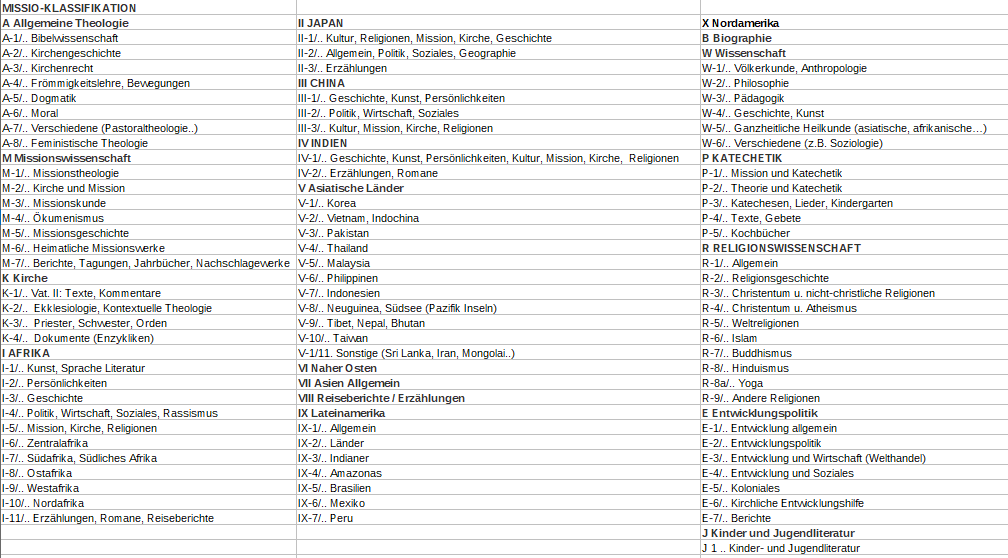
\includegraphics{img/img1.PNG}
\end{figure}

\textbf{Valentina de Toledo (VT): Thank you for your time and
availability to answer our questions. The library is a place where many
worlds meet, but also where patterns of the society in which it is
located are repeated, among them racism and other discriminations. I
would like to understand your view as an epistemologist and doctoral
student in Information Science on the impacts of whiteness in the field,
and in particular in Brazilian librarianship.}

\textbf{In the book \enquote{Epistemologias Latino-Americanas} (Latin American
Epistemologies) you say \enquote{Racism is a white issue, why only black people
should address it in their teaching and professional practice?} I would
like you to start by explaining what whiteness is?}

Franciéle Carneiro Garcês da Silva (FS): Ta-Nehisi Coates says \enquote{race is
the daughter of racism, not its mother} and from that I say in the book
that whiteness is \enquote{the mother of racism}. The concept of race was used
to classify people, be they from other continents or countries,
hierarchized into \enquote{superior and inferior races} in order to separate and
dominate. Whiteness refers to white racial identity that is
reconstructed according to local and global influences. The exercise of
whiteness was present when, in historical processes, European and
American white men used the concept of race to be able to colonize,
dominate, and enslave other people, as in the case of the African
population, and also to be able to justify the domination of these
populations using the pseudoscience of the time and religious aspects,
in addition to the power structure created.

By saying that whiteness is the mother of racism, I am not excluding
that people were already prejudiced before the concept of race, but when
it was invented, it served to classify and hierarchize people from
certain non-white groups. The white racial identity has since been
promoted as if there were \enquote{superior races}, and this racial privilege is
promoted in all spheres of Brazilian society.

And when I say that racism is a white problem, I am talking about a
conceptual model where whiteness according to historical processes is
responsible for what is seen today in Brazilian society as instruments
of domination of non-white people: the native/indigenous peoples, black
people of African origin, and the LGBTQIA population, who do not
correspond to the cisheterosexual hegemony. The aspects of domination
propagated by the elite that promotes whiteness act on the issues of
race, gender, class and sexuality and their intersectionality.

\textbf{VT: How is whiteness reflected in Brazilian society?}

FS: In Brazil, white people see themselves as having an alleged
normality, they see themselves as the standard to be reached. To be
white is, in their view, normal. Those who are different from the white
standard seek it as a way to achieve social status and be accepted in
society, either by whitening their features, appropriating discourses of
meritocracy and racial democracy, conforming to the white aesthetic by
straightening their hair, for example, or behaving in a certain way that
is not linked to the behavior of black and indigenous people.

Colonization in Brazil lasted a long time and colonial thinking
continues today. Here we have the perception that racist attitudes are
justifiable. You also have impediments to the development of black,
indigenous and LGBTQIA populations. And the ideal of whitening the
Brazilian population, a policy developed soon after abolition to bring
in white migrants from outside Brazil and mix the population that was
predominantly white at the time, so that over generations Brazilian
society would become white. This discourse is still exported outside
Brazil, where the referential of a Brazilian woman is Giselle Bündchen,
from the south of Brazil, a space where white ethno-racial groups
remained closed and related to each other. Many think that women from
Rio Grande do Sul are like her, when in fact we are very diverse.
Besides, with whitening there is a dilution of the knowledge of
ancestry, of religiosities, of African and Afro-Brazilian culture, of
capoeira, of samba. Elements of African origin that have already been
banned, as well as actions and manifestations of Afro-Brazilian
religiosity, such as Candomblé and Batuque, which were suppressed during
and after the slavery period, with laws to criminalize them, and even
today there are attacks by evangelicals on Umbanda and Candomblé
terreiros. The purpose is to destructure and remove this connection with
the ancestry of African people or people of African and Afro-Brazilian
origin, so that they can dominate and colonize their thinking and their
bodies.

It is important to understand that white people in Brazil are different
from white people in Europe or the USA. Also, a white person in the
south of Brazil is seen differently than a white person in the
northeast. Regardless of color, there are other aspects that make a
person be perceived as more or less white within this racialized society
of ours. Professors Lourenço Cardoso and Liv Sovik talk a lot about what
it is to be white in Brazil and what is the difference between these
expressions of whiteness.

\textbf{VT: How is it in the university context?}

FS: An evidence in Brazil of the expression of whiteness in academic
studies is through the racial quotas fraud, which are affirmative
actions for black and brown people. By using these ethno-racial quotas
to cheat quotas destined to native populations, quilombolas, or black
populations, because they think it is a privilege for these populations,
the white person exercises his whiteness, he cannot see himself as
belonging to the racial group that historically and socially is favored
and ignores (or pretends to ignore) the 300 years of slavery of black
people in Brazil. Black people who until today have not obtained any
return in the post-abolition of slavery, either material or immaterial
return or any public policy measure that would bring to these people
access to land or education.

\textbf{VT: Why can't white people see themselves in this favored
group?}

FS: One justification used is the myth of racial democracy, which says
that we are all equal. It justifies, along with meritocracy, that if
someone is not in a certain place it's due to their lack of his/her
effort, thus turns invisible the social and racial inequalities that are
remnants of historical processes. Why aren't there many black people in
universities today, even with quota policies? Why aren't there any black
professors at universities, even though there are public policies in
place to allow them to be there? If we all have the same intellectual
capacity and all possible abilities to exercise our profession in all
spaces, why aren't we the same or equal in number within the spaces of
power? This myth is a discourse created to unify the Brazilian
population in order to criminalize inequalities. Within the myth of
racial democracy you and I would be equal, but we see that even though
we are women, everything else is different: our place of birth,
families, the people we descend from, the opportunities in life we had,
so much so that today you are in Berlin and I am in Brazil. If we had
the same opportunities I would also be in Berlin or you would be in
Brazil. Opportunities for black women are very different from those for
white women.

From this there is also the myth of meritocracy, which is the question
of a merit created by whites, where we have to work hard in order to
grow, and then the growth will have been deserved. But how many times do
you see white people in positions of trust because they were indicated
by acquaintances? Or do you see them passing a public contest because
they know people on the board? The myth of meritocracy is only valid for
black or indigenous people. The profits of the slavery process did not
go into the pockets of black people who actually worked, but to white
people who did not work and unfairly obtained the monetary value of
someone else's work. In this reasoning, they don't deserve to have this
money, wealth, land, housing, et cetera, because they didn't work for
it.

And then there is racism, the existence in the social imaginary of
different races, with positive attributes for white people and negative
ones for black or indigenous people. Racism is promoted over contexts of
superior and inferior races; people who commit racism believe they are
superior. Without even realizing it, they dehumanize others through
offenses, actions, and violence that are often implied or unnoticed as
violence by those who suffer.

Another factor is the denial of rights. Why are black people today in
the greatest degree of inequality and social, economic, and educational
vulnerabilities? Because after the abolition of slavery, black people --
besides the repercussionsof the slavery process -- were denied their
rights (whether material, immaterial, or symbolic goods) by the State,
promoted by the lack of actions and public policies for them to develop
and rise socially, educationally, in short, to be better within a social
class?

Professor Kabengele Munanga says that racism in Brazil is effective
because what a person says cannot always be interpreted, it is
subliminal... In my perception, if something bothers or hurts a black
person, it is racism. However, it is not always possible to denounce
this kind of racism.

\textbf{VT: So, racism is exclusively exercised by white people?}

FS: White people perpetuate racism through perceptions and their
actions. That doesn't mean that black people can't reproduce -- and
that's the right word -- reproduce racism, because in a racist society
they learn that and reproduce it. If they don't have correct information
and don't dialogue in order to understand how race relations take place
in our society, they will continue reproducing the oppressor's discourse
forever, because society is racist. Black people in Brazil often don't
have access to their own history as belonging to the African population,
because all documents and records were basically destroyed and detonated
for fear that future generations would ask for redress of rights. The
myth of racial democracy means that they don't think that everything
that happens in their lives is because of racism, and they may think
that their lack of opportunities is because they don't try hard enough.

An important thing to understand, even brought up by professor Lia
Vainer Schucman, is that even if you are a very poor white person, you
will always have the privilege of color. It is a privilege that
structures the relations and makes you obtain opportunities, goods and
status within the Brazilian society.

\textbf{VT: What do you mean by racial privilege?}

FS: Racial privilege means reaping the benefits of whiteness, like a
poor white person being able to walk around in slippers in a certain
space without being thrown out by the security guard, or being seen as
an epistemic authority on a certain subject by touching on the topic
even without having studied it deeply. Not long ago, three white people
wrote an article about affirmative action issues and it was published,
and they don't work with that and wrote several absurd things in it.
Meanwhile, black people have their articles with ethno-racial discussion
refused, even with scientific production based on scientific
methodologies and other authors that approach the subject, under the
speech of being political, militant or radical.

This happens because we still have a model of science that is not
perceived as promoting white racial ideology. It is no wonder that we
don't have so many articles or books about the ethno-racial issue
published in Brazil in the library-economics-information field, unless
the books are published by white people talking about black people, and
few books written and published by black Brazilian people in our
context. The racial issue will always influence when a black person
talks about his experience, his side of the story, his critical
perspective and scientific evaluation, because, in case someone
evaluates the person when evaluating the material will be embedded with
the myth of racial democracy, meritocracy, whitening and racism.
Consequently, he will refute that production, either because he doesn't
understand anything about the subject or because he considers that
debate unnecessary, considering that he is in a society that is fair and
equal to all. This is the epistemicide, a concept widely discussed by
Boaventura de Sousa Santos and Sueli Carneiro, which consists in the act
of \enquote{killing} the knowledge produced by black people and others on the
margins, especially because it has a counter narrative to that produced
by the hegemonic context. It is no wonder that professors say they have
never read about ethnic-racial issues, or that a book was released in
2018 is the first on this discussion, when in fact the topic has been
discussed in Librarianship and Information Science for a long time.

\textbf{VT: And how does whiteness influence Librarianship and
Information Science (LIS)?}

FS: It has impacted librarianship in several ways.

First: by believing in the existence of different races, some being
considered as holders and producers of knowledge and others as neither
holders nor producers, as is the perception created about, for example,
the black population. It is as if these populations had no knowledge,
did not produce knowledge, nor reflected epistemologically about their
areas of knowledge and their social realities, of being and existence in
the world. Thus, a normative model of science is created that follows
the standards established in the global north.

Second: Librarianship in Brazil is a science that brought aspects of the
European and American strands, which promote what I would call White
Librarianship, and thus bring theoretical references and theories from
these regions, promoting, for the most part, a very Eurocentric
perspective of doing science, and which disregards all decolonial
knowledge and knowledge of people that are on the margins within this
society.

Putting these two influences together, we have epistemicide caused by
whiteness, the death of knowledge that is considered inferior within the
university. There are barriers built to people who want to discuss race
relations within librarianship through their course conclusion papers or
end-of-course research, with the argument that this discussion is not
considered something to be researched within our field.

There is an invisibilization of race and, by invisibilizing the issues
of race relations and among human beings, we have scenes like a teacher
following a teaching parameter of European models and thus not being
able to understand the situation and context of life of his students in
vulnerable situations, to put them, even if unconsciously, on the same
metric and evaluate them as if they came from equal opportunities, and
in Brazil this is not real.

\textbf{VT: Do teachers also exert their whiteness on students?}

FS: In the teaching profession, whiteness is present, as well as the
meritocratic thought and the myth of racial democracy in education. A
professor who thinks that everyone in the university comes from a
situation where it is common to have studied English, to have access to
know the types of articles, how to write them, among other things,
doesn't think about what took a person who didn't have this knowledge
and can't meet university standards to get into her/his classroom. And
there are professors who additionally give people low marks for not
understanding this other reality. A black person is not always prepared
to be in a university. There is, many times, an educational deficit
because we mostly come from public schools and when we get to the
university, there may be financial, educational, and even
interpretational difficulties to understand how this system works. There
is no informational literacy, for example, so that we arrive at the
university already knowing which parameters must be met and how to
maintain ourselves within this space, which is a historically white,
Eurocentered, Euro-americanized space. Not to mention the racist jokes
from professors, which I have often witnessed in my course, what we call
recreational racism, as the author Adilson Moreira says.

\textbf{VT: What is recreational racism?}

FS: Adilson Moreira shows in his book \enquote{Recreational Racism} that
recreational racism is based on racist jokes, like \enquote{the black person,
when he doesn't do it on the way in, he does it on the way out}, as if a
black person was always expected to do something wrong. The imaginary
has created this and attributes it to the racial-ethnic aspect, when in
fact any person can make mistakes regardless of being or not being a
black person.

\textbf{VT: What are the difficulties of understanding how the
university system works?}

FS: The barriers encountered by a black person in the university are,
for example, barriers of opportunity, the difficulty to be part of
research projects, extension projects, or to have (post)gradu\-ation
projects approved within a program because of their ethnic-racial
belonging or theme. It is important to understand that this is part of
subjectivities, a person who doesn't approve or doesn't consider an
opportunity to a black person doesn't necessarily do it knowing that
he/she is making a racial choice, this can be done in an unconscious way
for not having this perception or awareness that he/she is inside a
racist society.

The article \enquote{Whiteness in Teaching Practices in Librarianship and
Information Science}\footnote{\url{https://brapci.inf.br/index.php/res/v/102318}},
written by me, Gustavo Saldanha and Daniela Pizarro, is the only one
with this approach in ENACIB (National Meeting of Research in
Information Science), but the critical studies on whiteness have been
going on since the 2000s. The Afro-Canadian librarian and researcher
Jody Warner was the first to address the issue, followed by the teacher
and librarian Isabel Espinal, about whom Dirnéle Garcez and I wrote in
the book \enquote{Bibliotecári@s Negr@s -- v. 3} (Black Librarians,
\url{https://www.nyota.com.br/livros}) specifically about what Espinhal
recognizes and understands as whiteness in the library and information
science field.

\textbf{VT: Black people have the highest dropout rates in Brazilian
education (71.7\%), do you see whiteness having to do with that?}

FS: The evasion happens, many times, because they don't recognize
themselves in the librarianship course. People drop out because they
can't always afford it (since public universities also cost money, be it
transportation, food, rent or moving to another city) or because they
don't have the support that the university should give such as student
assistance programs, which are either non-existent or information is
difficult to access for black people. Another fact is that people who
can take the day off to study library science are privileged; many times
the night courses are the ones that black people will choose because
they work during the day and are providers.

On top of this there are racist attitudes that make black people feel
that this space is not theirs, they feel isolated, persecuted by
teachers, by colleagues, or by situations of institutional racism. And
without a welcome, be it a study group or a laboratory, professors or a
social worker from the university, the person is lost by evasion.

\textbf{VT: In teaching, do you use material from black or indigenous
Brazilians, or rather white Brazilians or people from the global north?}

FS: Many people who are references in our field are mostly white. When
we speak, for example, of epistemological and historical studies in LIS,
they are markedly white. We can cite among the references, the
professors: Gustavo Saldanha, César Karpinski, Solange Mostafa, Carlos
Alberto Ávila Araújo, Oswaldo Almeida Júnior, Henriette Gomes, among
others... Black references such as Maria Aparecida Moura, Mirian de
Aquino, Ana Cláudia Borges, Ana Paula Menezes, Leyde Klébia Rodrigues,
Francilene Cardoso, in short, all these black people are within the
production of knowledge, but are not always studied within the teaching
in Library Science in Brazil. However, they are within the works
published by black people who are librarians, such as the volumes of the
book \enquote{Bibliotecári@s Negr@s} and the book \enquote{O Negro na Biblioteca}, the
first ICB books related to the ethnic-racial issue.

In the spectrum of scientific production, one sees white people as the
most cited and recognized.

However, within the field there are white people who are evoking a
critical and humanities-oriented look within the
librarianship-information field, many of them, already mentioned above.
People you should definitely read when thinking about teaching
librarianship are Professor Francisco das Chagas Júnior and Professor
Daniella Pizarro, important references to understand the ethical aspects
of the profession and librarianship as an area that promotes a certain
technicality to the detriment of humanities. We can also mention
references such as Professor Jacqueline Cabral, archivologist who
studies archives, gender and sexuality in archivology, Professor
Henrriette, one of the theoretical bases to understand the social
protagonism within librarianship and IC; among others.

\textbf{VT: What do you mean by technicism?}

FS: We see a very strong strand within LIS in promoting ICTs
(Information and Communication Technologies) as those that should be
made visible in this century, while the humanities within our area are
left aside.

Professors Maria Aparecida Moura, Rubens Alves da Silva and Fabrício
Nascimento have promoted the humanities for the debate, at least here in
the UFMG {[}Universidade Federal de Minas Gerais{]}, and this is
important, because without the professors there is no movement in these
dialogues, since inside the university there is a fight for speeches,
for spaces of power, and usually black people are not visible in these
places, since whiteness is also promoted from the speeches of those who
want the debate as much as by those who do not want to follow this
direction.

\textbf{VT: Are perspectives from the humanities well accepted in LIS?}

FS: In my understanding, no. I see this in the resistance that exists
when you bring an uncomfortable subject to the white racial group,
precisely because it puts it in evidence and shows that those who
promote institutional, recreational, linguistic racism, among others,
are white people. It is still this group that will use its power to
remove black, indigenous, LGBTQIA and disabled people from their places
of enunciation, besides omitting and invisibilizing their existence and
their discourses within the academic spaces, so that they can continue
promoting a technicist librarianship, pseudo-neutral and propagator of a
supposed racial supremacy.

\textbf{VT: In your understanding, how is the library a \enquote{power space}
for the propagation of one racial group over another?}

FS: Imagine that there is a whole perspective on highlighting from
children's literature, which promotes Cinderella and Disney classics,
but does not turn its gaze to the African and Afro-Brazilian
literatures, indigenous literature, LGBTQIA literature to be included
within the libraries and information units, and mainly, to be in the
training spaces of professionals who will work with the population. To
me this is the promotion of a discourse in favor of whiteness, of racial
privilege and its maintenance that will always promote whiteness as the
standard.

\textbf{VT: How can you deal with that?}

FS: The information professional has to have a critical consciousness
about it and has to take a political attitude. I understand that
everything done in the training, in the curriculum and in the
performance is political. When I choose for a certain space a discourse
that invisibilizes the other, I take a political attitude. It can be
anti-racist, decolonial, political, or it can serve the molds of
capitalism, the hegemonic discourse of doing science, a literature that
promotes \enquote{a single history}, as Chimammanda Adichie says, and that
considers only white men as classics, while women are barely read, and
black women are not even known.

When we perceive this university, and when we perceive our place of
action, if we don't change this space we will always promote this
identity, this white racial privilege through what we read, do, say,
execute in our actions and as reflections within the science performed
in the area. It is very complex.

Changing university courses is a very strong movement, because you are
entering a high intellectual elite. In undergraduate courses, people who
are not connected to the racial debate often won't understand why this
is being discussed and why it is being included in professional
training. I have been in two universities where they did not understand
why we should include the discussion if our profession is a neutral
profession. This pseudo-neutrality is promoted in a very erroneous way.
For example: If you don't like black people, as a librarian who is to
say that you will not automatically provide the information that you
think a black person should receive and not a service that you would
provide if they were not a black person? When you don't serve a black
person because you consider a race inferior to your own, what is that if
not racism? In my understanding there is no way a person can be detached
from their particular values and beliefs, we are human beings and this
will eventually reflect in their work. This is why I say, based on
several authors that I have studied, that there is no professional
neutrality. We cannot talk about neutrality when people are socialized
in racist societies, when people are racialized and put into subordinate
categories because of the color of their skin. Learned prejudices are
carried into professional actions, whatever they may be, and the
librarian has to be aware of how this may affect his/her professional
sphere.

What has to be changed? Disciplines addressing ethno-racial, decolonial,
gender and sexuality issues should be included as a basis for all
librarianship courses, specified for the area, regardless of whether it
is a public or private university. A librarian has to become aware that
there are LGBTQIA people. It is not just because there is a name on the
card that the person is called by the name on the card. That deficit is
repeated and so you see how many librarians are conservative people.

\textbf{VT: In your chapters you explain about the models of LIS, and
the fact that the model used in Brazil is a technicist model, where
libraries are taken \enquote{as places of practicality, efficiency and
services}, and they see themselves as impartial. What is your idea
behind epistemic disobedience and} \emph{Critical Antiracist and
Decolonial Librarianship}\textbf{?}

FS: When I think about what I call Critical Antiracist and Decolonial
Librarianship, I think about how we keep promoting Eurocentric and
Americanized thinking and how we lack aperspective on our Brazilian
social and historical reality. Many librarians do not know the history
of Brazil, or they only know what they learned in school, and this lack
of knowledge causes the reproduction of the hegemonic discourse, the
discourse elaborated by those who colonized our population.

If there were decolonial references in universities, if knowledge within
librarianship education came from Latin women or Latin men, indigenous
people, riverine populations, quilombolas, if they had the perception of
race as an element that structures relations, The understanding of race
would not be so present in the imaginary construct of teachers,
employees, and classmates, groups would not be formed that exclude
people who are racialized, or abysses and difficulties would not be
created for people from vulnerable backgrounds or belonging to a
non-white ethno-racial group.

Decolonizing is looking at the knowledge produced by those on the
margins and it is considering this ecology of knowledge produced in the
global south. All of them can make our profession develop, become more
humanizing, there is more understanding, the other is more contemplated
in all the lessons we go through, regardless of being white, black or
indigenous. But let's think about all this population and think that
they do have their place of representation and representativeness within
our struggle.

Unfortunately what we still have, in my perception as an intellectual,
is a white European and American referential. In my publications I use
sources from white, indigenous, Asian, black, LGBTQIA people, whether
they are American, European, Brazilian, Latin American, but they all
identify this racial structure that promotes all the inequalities within
their places of work or their own countries, and that the library and
librarianship are spaces that promote this imagination, this colonized
white capitalist thinking. As a consequence, we have a white,
Americanized and European librarianship, which are not from our context
and do not have the same problems. Many times we evidence the thinking
of people who will not discuss race, will not discuss racism, will not
look at social and racial justice, because they are still based on the
myths of racial democracy and meritocracy.

Another form of epistemicide. If I'm a librarian who is not aware of the
racial issue within my actions and relationships, with no concept, no
understanding that race is part of all my work, and that it is within my
imagination, every time I select a work to be part of a collection or
not, I will always propagate this colonizing thought that I was taught,
and consequently, what I call white librarianship.

\textbf{VT: You talk about rethinking the Librarian Code of Ethics in an
explicitly anti-racist, anti-sexist, anti-LGBTQIA-phobic and decolonial
way for librarian conduct and also a direction for LIS courses. Could
you talk a little bit about the Code of Ethics?}

FS: My criticism of the code of ethics is that it doesn't bring a
perspective to reflect on race relations, and ignores them as an agenda
or element that causes tension among librarians. Black librarians
experience racism within their work environment, white librarians commit
racism within their work environment. The code of ethics should
instigate the librarian as a person, and that also requires thinking
about how it is produced by the federal council of librarianship. How
does the council think about the inclusion of the discussion about
ethnic-racial issues? How does it put that, as a librarian, it has to be
committed to the deconstruction of prejudices? Whether they are racial,
gender or sexual, and also deconstruct race as this social construct
within society? It is not enough to be intrinsic, it has to be explicit.
Very clear!

Basically what I want is the promotion of discussion about race by the
committees and how it influences the profession and you. From there it
is on to become an actor in raising awareness and deconstructing racism
within society.\footnote{Thanks to Arran Ridley for the comments and
  corrections.}

%autor
\begin{center}\rule{0.5\linewidth}{0.5pt}\end{center}

\textbf{Franciéle Carneiro Garcês da Silva}

\url{https://linktr.ee/FrancieleGarces}

Franciéle Carneiro Garcês da Silva is a doctoral student in information
Science at the Federal University of Minas Gerais. She works with
research and promotion of Brazilian and American Black Librarianship, as
well as decolonial studies and teaching, critical race theory, and
critical studies of whiteness at LIS. Among her many projects, she is
manager of the Intellectual Quilombo and coordinator of the Nyota Seal,
organizer and writer of many books, including: Black Librarians (with 3
volumes), Black Epistemologies: race relations in librarianship and
Latin American Epistemologies in Library and information science:
contributions from Colombia and Brazil.

\textbf{Valentina Gonçalves de Toledo}

Valentina Gonçalves de Toledo is a Brazilian Library and Information
Science student in the Humboldt-University Berlin.

\newpage

\hypertarget{o-racismo-uxe9-uma-problemuxe1tica-branca-por-que-somente-pessoas-negras-suxe3o-aquelas-que-deveriam-aborduxe1-lo-em-sua-pruxe1tica-docente-e-profissional}{%
\section[\enquote{O racismo é uma problemática \textit{branca}, por que somente
pessoas negras são aquelas que deveriam abordá-lo em sua prática docente
e profissional?}]{\enquote{O racismo é uma problemática \textit{branca}, por que somente
pessoas negras são aquelas que deveriam abordá-lo em sua prática docente
e profissional?}}\label{o-racismo-uxe9-uma-problemuxe1tica-branca-por-que-somente-pessoas-negras-suxe3o-aquelas-que-deveriam-aborduxe1-lo-em-sua-pruxe1tica-docente-e-profissional}}
\subsection*{Bibliotecária Franciéle Garcês conta sobre a influência da branquitude
no campo biblioteconômico-informacional e a perpetuação do racismo na
biblioteconomia e ciência da informação.}

\begin{figure}[h!]
\centering
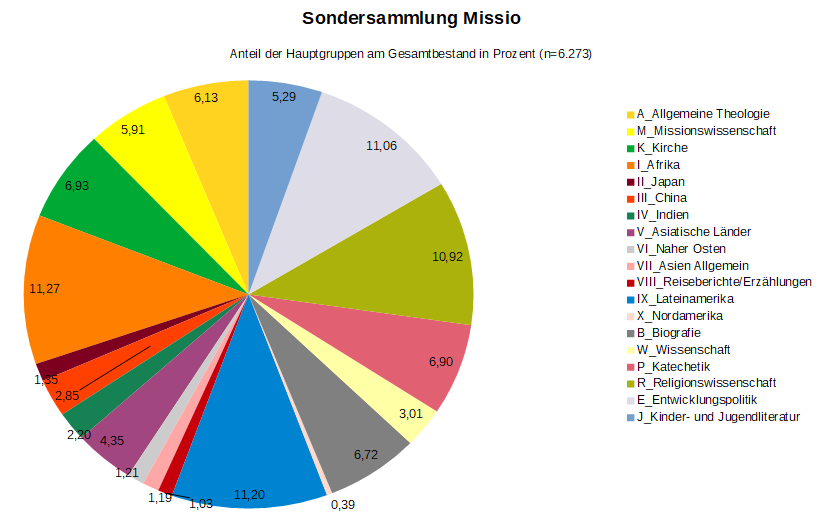
\includegraphics{img/img2.PNG}
\end{figure}

\textbf{Valentina de Toledo (VT): Obrigada pelo seu tempo e pela
disponibilidade em responder nossas perguntas. A biblioteca é um lugar
onde muitos mundos se encontram, mas também onde padrões da sociedade na
qual ela se localiza se repetem, entre eles o racismo e outras
discriminações. Nós gostaríamos de entender sua visão como epistemóloga
e doutoranda em Ciência da Informação sobre os impactos da branquitude
na área, e em especial na biblioteconomia brasileira.}

\textbf{No livro \enquote{Epistemologias Latino-Americanas} você diz
\enquote{o Racismo é uma problemática branca, por que somente pessoas
negras são aquelas que deveriam abordá-lo em sua prática docente e
profissional?}. Gostaria que você começasse falando sobre o que é a
branquitude?}

Franciéle Carneiro Garcês da Silva (FS): Ta-Nehisi Coates diz \enquote{a
raça é a filha do racismo, não a sua mãe} e a partir disso digo no livro
que branquitude é \enquote{a mãe do racismo}. O conceito de raça foi
usado para classificar pessoas, sejam elas de outros continentes ou
países, hierarquizadas em \enquote{raças superiores e inferiores} a fim
de separar para dominar. A branquitude se refere à identidade racial
branca que se reconstrói conforme as influências locais e globais. O
exercício da branquitude esteve presente quando, em processos
históricos, homens brancos europeus e americanos utilizaram o conceito
de raça para poder colonizar, dominar e escravizar outros povos, como no
caso da população africana, e também para poder justificar a dominação
dessas populações utilizando a pseudociência da época e os aspectos
religiosos, além da estrutura de poder criada.

Ao dizer que a branquitude é a mãe do racismo, não excluo que as pessoas
já eram preconceituosas antes do conceito de raça, mas ao ser inventado,
ele serviu para classificar e hierarquizar pessoas de determinados
grupos não-brancos. A identidade racial branca desde então se promove
como se existissem \enquote{raças superiores}, e esse privilégio racial
se promove em todas as esferas da sociedade brasileira.

E ao falar que racismo é uma problemática branca, eu falo de um modelo
conceitual onde a branquitude consoante aos processos históricos é
responsável pelo que hoje se vê na sociedade brasileira como
instrumentos de dominação de povos não brancos: os povos
originários/indígenas, negros de origem africana, e população LGBTQIA,
que não correspondem à hegemonia cisheterossexual. Os aspectos de
dominação propagados pela elite que promove a branquitude atuam nas
questões de raça, gênero, classe e sexualidade e suas
interseccionalidades.

\textbf{VT: E como é a branquitude no Brasil?}

FS: No Brasil, as pessoas brancas se veem como detentoras de uma
normalidade não existente, elas se veem como o padrão a ser alcançado.
Ser branco é, a seu ver, o normal. Quem se difere do padrão branco o
busca como um meio de alcançar um status social e ser aceito dentro da
sociedade, seja por meio de branqueamento de suas feições, apropriação
de discursos meritocráticos e de democracia racial, adequação à estética
branca com o alisamento do seu cabelo, por exemplo, ou se portar de uma
certa maneira que não seja vinculada ao comportamento de pessoas negras
e indígenas.

A colonização no Brasil durou muito tempo e o pensamento colonial
continua até hoje. Aqui se tem a percepção de que atitudes racistas são
justificáveis. Também se tem impeditivos para que as populações negra,
indígena e LGBTQIA se desenvolvam. E o ideal do branqueamento da
população brasileira, política elaborada logo após a abolição, para
trazer migrantes brancos de fora do Brasil e miscigenar a população que
era predominantemente à época, para que com o passar das gerações a
sociedade brasileira se tornasse branca. Esse discurso ainda é exportado
para fora do Brasil, onde o referencial de mulher brasileira é Giselle
Bündchen, oriunda do sul do Brasil, um espaço onde grupos étnico-raciais
brancos se mantiveram fechados e relacionaram-se entre si. Muitos acham
que mulheres do Rio Grande do Sul são como ela, quando na verdade somos
muito diversas. Além disso, com o branqueamento se tem uma diluição do
conhecimento de ancestralidade, das religiosidades, da cultura africana
e afro-brasileira, da capoeira, do samba. Elementos de origem africana
que já foram proibidos, assim como ações e manifestações de
religiosidade afro-brasileiras, como o Candomblé e o Batuque, as quais
foram suprimidas durante e após o período da escravidão, com leis para
criminalizá-las, e até hoje há ataques de evangélicos aos terreiros de
umbanda e candomblé. O propósito é desestruturar e retirar essa conexão
com a ancestralidade de pessoas africanas ou de origem africana e
afro-brasileira, pois assim conseguem dominar e colonizar o pensamento e
seus corpos.

É importante entender que pessoas brancas no Brasil são diferentes de
pessoas brancas na Europa ou nos EUA. Além disso, uma pessoa branca no
sul do Brasil é vista diferentemente de uma pessoa branca no nordeste.
Independentemente da cor, há outros aspectos que a fazem ser entendida
como mais ou menos branca dentro dessa nossa sociedade que é
racializada. Os professores Lourenço Cardoso e Liv Sovik falam muito
sobre o que é ser branco no Brasil e qual a diferença dessas expressões
da branquitude.

\textbf{VT: Como é no contexto universitário?}

FS: Um parâmetro de demonstração atual no Brasil de expressão da
branquitude no estudo acadêmico é através da fraude de cotas raciais,
que são ações afirmativas para pessoas negras e pardas. Ao se utilizar
dessas cotas étnico-raciais para fraudar cotas destinadas à populações
originárias, quilombolas ou populações negras por achar um privilégio
para essas populações, a pessoa branca exerce a sua branquitude, ela não
consegue se olhar quanto pertencente ao grupo racial que histórica e
socialmente é favorecido e ignora (ou finge ignorar) os 300 anos de
escravidão de populações negras no Brasil. Povos negros que até hoje não
obtiveram retorno no pós-abolição da escravatura, seja o retorno
material, imaterial ou alguma medida de política pública que trouxesse a
essas pessoas acesso à terra ou à educação.

\textbf{VT: Por que pessoas brancas não conseguem se ver nesse grupo
favorecido?}

FS: Uma justificativa utilizada é o mito da democracia racial, que fala
que todos somos iguais. Justifica, junto à meritocracia, que se alguém
não está em determinado lugar é devido à sua falta de esforço,
invisibilizando, assim, as desigualdades sociais e raciais que são
resquícios de processos históricos. Por que não tem tantos negros hoje
dentro da universidade mesmo com políticas de cotas? Por que não tem
professores negros dentro da universidade mesmo existindo políticas
públicas para que eles possam estar lá? Se todos temos a mesma
capacidade intelectual e todas as capacidades possíveis para exercer a
nossa profissão em todos os espaços, por que que nós não somos iguais ou
não estamos em número iqualitário dentro dos espaços de poder? Esse mito
é um discurso criado para unificar a população brasileira a fim de
criminalizar as desigualdades. Dentro do mito da democracia racial você
e eu seríamos iguais, mas vemos que mesmo sendo mulheres, todo resto é
diferente: o lugar de nascimento, famílias, povos dos quais descendemos,
oportunidades na vida que tivemos, tanto que hoje você está em Berlim e
eu estou no Brasil. Se tivéssemos a mesma oportunidade eu também estaria
em Berlim ou você no Brasil. Oportunidades para mulheres negras são
muito diferentes daquelas destinadas às mulheres brancas.

A partir disso há também o mito da meritocracia, que é a questão de um
merecimento criado pelos brancos, onde temos de nos esforçar para
conseguir crescer e, assim, o crescimento terá sido merecido. Mas
quantas vezes não se vê pessoas brancas em cargos de confiança porque
foram indicadas por conhecidos? Ou se vê elas passarem em concurso
público por conhecerem pessoas da banca? O mito da meritocracia só vale
para pessoas negras ou indígenas. A herança do processo escravista não
foi para o bolso das pessoas negras que trabalharam de fato, mas sim
para pessoas brancas que não trabalharam e obtiveram de forma injusta o
valor monetário do trabalho de outrem. Nesse raciocínio, eles não
mereceriam estar com esse dinheiro, riquezas, terra, moradia, etc., pois
não foram eles quem trabalharam para obtê-los.

E ainda tem o racismo, a existência no imaginário social de raças
diferentes, com atributos positivos para pessoas brancas e negativos
para pessoas negras ou indígenas. O racismo se promove em cima de
contextos de raças superiores e inferiores, pessoas que cometem racismo
acreditam ser superiores. Mesmo sem perceber, elas desumanizam as outras
por intermédio de ofensas, ações e violências, que diversas vezes são
subentendidas ou passam despercebidas como violência por aqueles que
sofrem.

Outro fator é a negação de direitos. Por que as pessoas negras hoje
estão no maior grau de desigualdade e vulnerabilidades sociais,
econômicas e educacionais? Por que após a abolição da escravatura,
pessoas negras - além das sequelas do processo de escravidão -, tiveram
a negação de direitos (sejam eles bens materiais, imateriais ou
simbólicos) pelo Estado promovida pela falta de ações e de políticas
públicas para que se desenvolvessem e ascendessem socialmente,
educacionalmente, enfim, estivessem melhor dentro de uma classe social?

O professor chamado Kabengele Munanga diz que o racismo no Brasil é
efetivo, porque nem sempre aquilo que a pessoa fala pode ser
interpretado, é subliminar\ldots{} Na minha percepção, se algo incomoda
ou se magoa uma pessoa negra é racismo e acabou. No entanto, nem sempre
é possível fazer uma denúncia contra esse tipo de racismo.

\textbf{VT: Racismo é então exercido exclusivamente por pessoas
brancas?}

FS: As pessoas brancas perpetuam o racismo através de percepções e das
suas ações. Isso não quer dizer que pessoas negras não possam reproduzir
- e essa é a palavra correta -, reproduzir o racismo, porque dentro de
uma sociedade racista elas aprendem aquilo e reproduzem. Se não tiverem
informação correta e não dialogarem para entender como se dão as
relações raciais na nossa sociedade, seguirão reproduzindo o discurso do
opressor para sempre, pois a sociedade é racista. Pessoas negras no
Brasil, muitas vezes, não têm acesso à sua própria história enquanto
pertencentes à população africana, porque todos os documentos e
registros foram basicamente destruídos e detonados por medo de que as
gerações futuras pedissem reparação de direitos. O mito da democracia
racial faz com que elas não achem que tudo que acontece na vida delas
seja por conta de racismo, e podem achar que a falta de oportunidades se
dá por não se esforçarem o suficiente.

Uma coisa importante de entender, inclusive trazido pela professora Lia
Vainer Schucman, é que mesmo sendo uma pessoa branca bem pobre, você
sempre vai ter o privilégio da cor. É um privilégio que estrutura as
relações e faz com que se obtenha oportunidades, bens e status dentro da
sociedade brasileira.

\textbf{VT: O que você quer dizer com privilégio racial?}

FS: Um privilégio racial significa colher os benefícios da branquitude,
como uma pessoa pobre branca poder andar de chinelo dentro de um
determinado espaço sem ser colocada para fora pelo segurança, ou ser
vista como uma autoridade epistêmica sobre um determinado assunto ao
tocar no tema mesmo sem tê-lo estudado profundamente. Há pouco tempo,
três pessoas brancas escreveram um artigo sobre questões de ações
afirmativas e ele foi publicado, sendo que não trabalham com isso e
escreveram várias coisas absurdas nele. Enquanto isso, pessoas negras
têm os artigos com discussão étnico-racial recusados, mesmo com produção
científica baseada em metodologias científicas e outros autores que
abordam o assunto, sob o discurso de estarem sendo políticos, militantes
ou radicais.

Isso acontece porque ainda temosum modelo de ciência que não se percebe
como promotor da ideologia racial branca. Não é à toa que não se tem
tantos artigos nem livros sobre a questão étnico-racial publicados no
Brasil no campo biblioteconômico-informacional, a não ser que os livros
sejam publicados por pessoas brancas a falar sobre negros, e poucos são
os livros escritos e publicados por pessoas negras brasileiras em nosso
contexto. A questão racial vai sempre influenciar quando uma pessoa
negra fala sobre sua experiência, o seu lado da história, sua
perspectiva crítica e avaliação científica, pois, caso alguém avalie, a
pessoa ao avaliar o material estará embutida do mito da democracia
racial, da meritocracia, do branqueamento e do racismo. Consequentemente
refutará aquela produção, seja por não entender nada do assunto ou por
considerar aquele debate desnecessário por considerar que está em uma
sociedade que é justa e igualitária a todos. Isso é o epistemicídio, um
conceito muito debatido por Boaventura de Sousa Santos e Sueli Carneiro,
que consiste no ato de \enquote{matar} o conhecimento produzido por
pessoas negras e outras às margens, especialmente, porque e possui uma
contra-narrativa fora daquela produzida pelo contexto hegemônico. Não é
à toa que professores dizem nunca ter lido sobre questões
étnico-raciais, ou que um livro foi lançado em 2018 é o primeiro sobre
essa discussão, quando na verdade o tema já é discutido na
Biblioteconomia e Ciência da Informação há muito tempo.

\textbf{VT: E como a branquitude influencia a Biblioteconomia e Ciência
da Informação (BCI)?}

FS: Na biblioteconomia a sua influência ocorre de diversas formas.

Primeiro: ao acreditar na existência de raças diferentes, sendo umas
consideradas detentoras e produtoras de conhecimento e outras como nem
detentoras e tampouco produtoras, como é a percepção criada sobre, por
exemplo, a população negra. É como se essas populações não tivessem
saberes, não produzissem conhecimento, nem refletissem
epistemologicamente sobre suas áreas de conhecimento e suas realidades
sociais, de ser e estar no mundo. Assim se cria um modelo normativo de
ciência que segue os padrões estabelecidos no norte global.

Segundo: A biblioteconomia no Brasil é uma ciência que trouxe aspectos
das vertentes europeias e estadunidense, que promovem o que eu chamaria
de Biblioteconomia Branca, e assim trazem referenciais teóricos e
teorias vindos dessas regiões, promovem, em sua maioria, uma perspectiva
muito eurocentrada de fazer ciência, e que desconsidera todos os saberes
decoloniais e saberes de pessoas que estão à margem dentro dessa
sociedade.

Juntando essas duas influências, têm-se epistemicídio causado pela
branquitude, a morte de conhecimentos que são tidos como inferiores
dentro da universidade. Há barreiras construídas às pessoas que querem
discutir relações raciais dentro da biblioteconomia por intermédio dos
seus trabalhos de conclusões de cursos ou pesquisas de conclusão de
curso, com o argumento dessa discussão não ser considerada algo a ser
pesquisado dentro da nossa área.

Tem uma invisibilização da raça e, ao invisibilizar as questões das
relações raciais e entre seres humanos, se têm cenas como um professor
seguir um parâmetro de ensino de modelos europeus e assim não conseguir
entender a situação e contexto de vida de seus alunos em situação de
vulnerabilidades, de colocá-los, mesmo que inconsciente, sobre a mesma
métrica e avaliá-los como se viessem de oportunidades iguais, sendo que
no Brasil isso não é real.

\textbf{VT: Docentes também exercem sua branquitude sobre os alunos?}

FS: Dentro do exercício docente, a branquitude é presente, assim como o
pensamento meritocrático e do mito da democracia racial no ensino. Um
professor que acha que todas as pessoas na universidade vêm de uma
situação em que se é comum ter estudado inglês, ter acesso a saber os
tipos de artigos, como escrevê-los, entre outras coisas, não pensa sobre
o que levou uma pessoa que não teve esses conhecimentos e não consegue
atender aos padrões universitários. E há professores que, além disso,
dão nota baixa às pessoas por não entenderem essa outra realidade. Uma
pessoa negra nem sempre é preparada para estar em uma universidade. Há,
muitas vezes, um déficit escolar porque viemos na grande maioria de
escolas públicas e quando se chega à universidade, pode haver
dificuldades financeiras, educacionais e até mesmo de entender como esse
sistema funciona. Não há um letramento informacional, por exemplo, para
que cheguemos à universidade já sabendo quais são os parâmetros que
devem ser atendidos e como se manter dentro desse espaço, que é
historicamente branco, eurocentrado, euroamericanizado. Sem contar as
piadas racistas de docentes, que muitas vezes já presenciei no meu
curso, o que a gente chama de racismo recreativo, como diz o autor
Adilson Moreira.

\textbf{VT: O que é racismo recreativo?}

FS: O Adilson Moreira em seu livro \enquote{Racismo Recreativo} mostra
que o racismo recreativo é pautado por intermédios de brincadeiras
racistas, como \enquote{o negro quando não faz na entrada, faz na
saída}, como se esperasse que uma pessoa negra sempre fizesse algo de
errado. O imaginário criou isso e atribui ao aspecto étnico-racial,
quando na verdade qualquer pessoa pode cometer erros independentemente
deser ou não uma pessoa negra.

\textbf{VT: Quais são as dificuldades de entender como o sistema
universitário funciona?}

FS: As barreiras encontradas por uma pessoa negra dentro da universidade
são por exemplo: barreiras de oportunidades, a dificuldade de fazer
parte de projetos de pesquisa, projetos de extensão, ou de ter projetos
de (pós-)graduação aprovados dentro de um programa por conta de seu
pertencimento ou tema étnico-racial. É importante entender que isso faz
parte de subjetividades, uma pessoa que não aprova ou não considera uma
oportunidade a uma pessoa negra não necessariamente o faz sabendo que
está fazendo uma escolha racial, isso pode ser feito de forma
inconsciente por não ter essa percepção ou consciência de que está
dentro de uma sociedade racista.

O Artigo \enquote{A Branquitude nas Práticas Docentes em Biblioteconomia
e Ciência da Informação}\footnote{\url{https://brapci.inf.br/index.php/res/v/102318}},
escrito por mim, Gustavo Saldanha e Daniela Pizarro, é o único com essa
abordagem no ENACIB (Encontro Nacional de Pesquisa em Ciência da
Informação), mas os estudos críticos da branquitude já vêm desde os anos
2000. A bibliotecária e pesquisadora afro-canadense Jody Warner foi a
primeira a abordar o tema, a seguir a professora e bibliotecária Isabel
Espinal, sobre a qual inclusive Dirnéle Garcez e eu escrevemos no livro
\enquote{Bibliotecári@s Negr@s - v. 3}
(\url{https://www.nyota.com.br/livros}), especificamente sobre o que
Espinhal reconhece e entende como branquitude no campo
biblioteconômico-informacional.

\textbf{VT: Os maiores índices de evasão no ensino brasileiro são de
pessoas negras (71,7\%), você pensa que a branquitude tem a ver com
isso?}

FS: A evasão se dá, muitas vezes, por não se reconhecerem no curso de
biblioteconomia. As pessoas desistem porque nem semprepodem pagar (visto
que a universidade pública também custa, seja transporte, alimentação,
aluguel ou mudança de cidade) ou porque não têmo suporte que a
universidade deveria dar, como programas de assistência estudantil, que
ou é inexistente ou a informação é de difícil acesso para pessoas
negras. Outro fato é que pessoas que podem ter o dia para cursar
biblioteconomia são privilegiadas, muitas vezes os cursos noturnos são
aqueles que as pessoas negras irão escolher porque elas trabalham
durante o dia e são arrimo de família.

No topo disso tem atitudes racistas que fazem com que as pessoas negras
achem que esse espaço não é delas, sentem-se isoladas, perseguidas por
docentes, por colegas, ou por situações de racismo institucional. E sem
um acolhimento, seja um grupo de estudo ou laboratório, professores ou
assistente social da universidade, se perde a pessoa por evasão.

\textbf{VT: No ensino do Brasil se usa material de pessoas negras ou
indígenas brasileiras , ou mais de pessoas brancas brasileiras ou do
norte global?}

FS: Muitas pessoas que são referências dentro da nossa área são em sua
maioria brancas. Quando se fala, por exemplo, de estudos epistemológicos
e históricos na BCI, eles são marcadamente brancos. Podemos citar entre
as referências, os professores: Gustavo Saldanha, César Karpinski,
Solange Mostafa, Carlos Alberto Ávila Araújo, Oswaldo Almeida Júnior,
Henriette Gomes, entre outros\ldots{} Referências negras como Maria
Aparecida Moura, Mirian de Aquino, Ana Cláudia Borges, Ana Paula
Menezes, Leyde Klébia Rodrigues, Francilene Cardoso, enfim, todas essas
pessoas negras estão dentro da produção do conhecimento, mas nem sempre
são estudadas dentro da Biblioteconomia no Brasil. No entanto, estão
dentro das obras publicadas por pessoas negras que são bibliotecárias,
como os volumes do livro \enquote{Bibliotecári@s Negr@s} e no livro
\enquote{O Negro na Biblioteca}, primeiros livros de BCI relacionados à
questão étnico-racial.

No espectro de produção científica, vê-se as pessoas brancas como as
mais citadas e reconhecidas.

No entanto, dentro do campo há pessoas brancas que estão evocando um
olhar crítico e voltado para as humanidades dentro do campo
biblioteconômico-informacional, muitas delas, inclusive já citadas
acima. Pessoas que não se pode deixar de ler quando se pensa no ensino
de biblioteconomia é o professor Francisco das Chagas Júnior e a
professora Daniella Pizarro, importantes referências para entender os
aspectos éticos da profissão e a Biblioteconomia enquanto uma área que
promove um certo tecnicismo em desfavor das humanidades. Podemos citar
ainda, referencias como a professora Jacqueline Cabral, arquivologista
que estuda arquivos, gênero e sexualidade na Arquivologia, a professora
Henrriette, uma das bases teóricas para entender o protagonismo social
dentro da biblioteconomia e CI; entre outros

\textbf{VT: O que você quer dizer com tecnicismo?}

FS: Vemos uma vertente muito forte dentro da BCI na promoção das TICs
(Tecnologias da Informação e Comunicação) como aquelas que devem ser
visibilizadas neste século, enquanto as humanidades dentro da nossa área
são deixadas de lado.

Os professores Maria Aparecida Moura, Rubens Alves da Silva e Fabrício
Nascimento promoveram as humanidades para o debate, pelo menos aqui na
UFMG, e isso é importante, porque sem os professores não há movimentação
nesses diálogos, já que dentro da universidade ocorre briga por
discursos, por espaços de poder, e geralmente pessoas negras não são
visibilizadas nesses lugares, já que a branquitude também se promove a
partir dos discursos dos que querem o debate tanto quanto dequem não
quer seguir essa direção.

\textbf{VT: Essa visão humanista é bem aceita na BCI?}

FS: No meu entendimento, não. Percebo isso na resistência que há quando
se traz um tema desconfortável para o grupo racial branco, justamente
por colocá-lo em evidência e mostrar que quem promove o racismo
institucional, recreativo, linguístico, entre outros, são as pessoas
brancas. É ainda esse grupo que vai utilizar do seu poder para retirar
pessoas negras, indígenas, LGBTQIA, população com deficiência de seus
lugares de enunciação, além de omitir e invisibilizar suas existências e
seus discursos dentro dos espaços acadêmicos, para que assim, continue a
promoção de uma biblioteconomia tecnicista, pseudoneutra e propagadora
de uma suposta supremacia racial.

\textbf{VT: No seu entendimento, como a biblioteca é um \enquote{espaço
de poder} para a propagação de um grupo racial em detrimento de outro?}

FS: Imagine que há toda uma perspectiva em evidenciar desde a literatura
infantojuvenil, que promove Cinderela e clássicos da Disney, mas não
volta o seu olhar para que as literaturas africana e afro-brasileira,
literatura indígena, literatura LGBTQIA sejam incluídas dentro das
bibliotecas e das unidades de informação e, principalmente, estarem nos
espaços de formação de profissionais que vão trabalhar com a população.
Isso para mim é a promoção de um discurso em favor da branquitude, do
privilégio racial e de sua manutenção que vai sempre promover o branco
como padrão.

\textbf{VT: Como é possível lidar com isso?}

FS:O profissional de informação tem que ter uma consciência crítica a
respeito disso e precisa tomar uma atitude política. Eu entendo que tudo
que é na formação, no currículo e na sua atuação é algo político. Quando
eu escolho para um determinado espaço um discurso que invisibiliza o
outro, eu tomo uma atitude política. Ela pode ser antirracista,
decolonial, política ou pode servir aos moldes do capitalismo, ao
discurso hegemônico de fazer ciência, a uma literatura que promove
\enquote{uma história única}, como diz Chimammanda Adichie, e que
considera só homens brancos como clássicos, enquanto as mulheres mal se
lê, e mulheres negras nem se sabe quaem são.

Quando nós percebemos essa universidade, e quando percebemos o nosso
lugar de atuação, se não mudamos esse espaço promoveremos sempre essa
identidade, esse privilégio racial branco por intermédio daquilo que
lemos, fazemos, dizemos, executamos em nossas ações e enquanto reflexões
dentro da ciência realizada na área. É bem complexo.

Alterar os cursos da universidade é um movimento muito forte, porque se
entra numa alta elite intelectual. Nos cursos de graduação, pessoas que
não estão vinculadas ao debate racial muitas vezes não vão entender o
porquê de colocar isso em debate e na formação profissional. Eu já
passei por duas universidades onde não entenderam porque incluir a
discussão se a nossa profissão é uma profissão neutra. Essa
pseudoneutralidade é promovida de uma forma muito errônea. Por exemplo:
Se você não gosta de pessoas negras, como bibliotecária, quem garante
que você não irá automaticamente fornecer a informação que você acha que
uma pessoa negra tem que receber e não um serviço que você ofereceria se
ela não fosse uma pessoa negra? Quando você não atende uma pessoa negra
por considerar uma raça inferior à sua, o que é isso se não o racismo?
No meu entendimento não tem como uma pessoa se desvincular dos seus
valores e crenças particulares, somos seres humanos e isso eventualmente
irá refletir no seu trabalho. É por isso que eu digo, baseada em vários
autores que tenho estudado, que não existe neutralidade profissional.
Não podemos falar de neutralidade quando as pessoas são socializadas em
sociedades racistas, quando as pessoas são racializadas e colocadas em
categorias de subordinação por causa da cor de sua pele. Os preconceitos
aprendidos são levados para as ações profissionais, sejam elas quais
forem, e a bibliotecária tem que ter consciência de como isso pode
afetar sua esfera profissional.

O que tem de ser mudado? Disciplinas abordando questões étnico-raciais,
decolonialidades, de gênero e sexualidade deveriam ser incluídas como
base para todos os cursos de biblioteconomia, específicos para a área,
independentemente de ser universidade pública ou particular. Um
bibliotecário tem de se sensibilizar que existem pessoas transgêneros,
LGBTQIA, lésbicas, não-binárias. Não é só porque tem um nome na carteira
que a pessoa se chama pelo nome da carteira. Esse déficit se repete e
por isso se vê como muitas bibliotecárias são pessoas conservadoras.

\textbf{VT: Nos seus capítulos você explica sobre os modelos de BCI, e o
fato de o modelo usado no Brasil ser um modelo tecnicista, onde
bibliotecas são tomadas \enquote{como lugares de praticidade, eficiência
e serviços}, além de se verem como imparciais. Qual é a sua ideia por
trás da desobediência epistêmica e da Biblioteconomia Crítica
Antirracista e Decolonial (BCAD)?}

FS: Quando eu penso no que chamo de Biblioteconomia Crítica Antirracista
e Decolonial \linebreak (BCAD), penso em como continuamos promovendo o pensamento
eurocentrado e americanizado e como nos falta olhar para a nossa
realidade social e histórica brasileira. Muitos bibliotecários não
conhecem a história do Brasil, ou só conhecem a aprendida na escola, e
essa falta de conhecimento causa a reprodução do discurso hegemônico, o
discurso elaborado por quem colonizou a nossa população.

Se houvessem referênciass decoloniais em universidades, se o
conhecimento dentro do ensino de biblioteconomia fosse oriundo de
mulheres latinas ou homens latinos, pessoas indígenas, populações
ribeirinhas, quilombolas, se tivessem a percepção de raça como um
elemento que estrutura as relações, conhecimento de teorias
africanas\ldots{} O entendimento de raça não estaria tão presente na
construção do imaginário de docentes, funcionários e colegas de aula,
não se formariam grupos que excluem pessoas que são racializadas ou não
se criariam abismos e dificuldades para pessoas de origem vulnerável ou
pertencentes a um grupo étnico-racial não-branco.

Decolonizar é olhar para o conhecimento produzido por aqueles à margem e
é considerar essa ecologia de conhecimentos produzidos no sul global.
Todos eles podem fazer com que a nossa profissão se desenvolva, se torne
mais humanizada, haja mais compreensão, o outro seja mais contemplado em
todas as lições que a gente passa, independentemente de ser branco,
negro ou indígena. Mas que se pense em toda essa população e pense que
ela tem sim que ter o seu lugar de representação e representatividade
dentro da nossa luta.

Infelizmente o que ainda se tem, na minha percepção enquanto
intelectual, é um referencial branco europeu e americano. Nas
publicações utilizo fontes de pessoas brancas, indígenas, asiáticas,
pretas, LGBTQIA, sejam elas americanas, europeias, brasileiras, da
América Latina, mas todas elas identificam essa estrutura racial que
promove todas as desigualdades dentro de seus lugares de atuação ou seus
próprios países, e que a biblioteca e a biblioteconomia são espaços que
promovem esse imaginário, esse pensamento branco capitalista colonizado.
Como consequência temos uma biblioteconomia branca, americanizada e
europeia, que não são do nosso contexto e não possuem as mesmas
problemáticas. Muitas vezes evidenciamos um pensamento de pessoas que
não vão discutir raça, não discutem racismo, não olham para justiça
social e racial, porque ainda estão pautadas nos mitos da democracia
racial e na meritocracia.

Mais uma forma de epistemicídio. Se eu sou uma bibliotecária que não
está consciente da \linebreak questão racial dentro das minhas ações e relações,
sem conceito, entendimento de que raça faz parte de todo o meu fazer, e
que é ela que está dentro do meu imaginário, cada vez que selecionar uma
obra para fazer ou não parte de um acervo eu vou sempre propagar esse
pensamento colonizador para o qual fui ensinada, e por consequência, o
que chamo de biblioteconomia branca.

\textbf{VT: Você fala sobre repensar o Código de Ética Bibliotecário de
forma explicitamente antirracista, antissexista, anti-LGBTQIAfobico e
decolonial para a conduta bibliotecária e também de um direcionamento
para cursos de BCI. Você poderia falar um pouco sobre o Código de
Ética?}

FS: A minha crítica ao código de ética é por ele não trazer uma
perspectiva de refletir sobre as relações raciais, além de ignorá-las
como pauta ou elemento que causa tensão entre bibliotecários.
Bibliotecários negros sofrem racismo dentro de seu ambiente de trabalho,
bibliotecários brancos cometem racismo dentro do seu ambiente de
trabalho. O código de ética deveria instigar o bibliotecário, e isso
requer também pensar como ele é produzido pelo Conselho Federal de
Biblioteconomia. Como o conselho pensa a inclusão da discussão sobre
questões étnico-raciais? Como colocar que, enquanto bibliotecário, tem
de se comprometer com a desconstrução de preconceitos? Sejam eles de
ordem racial, de gênero ou sexualidade, e também desestruturar a raça
enquanto esse construto social dentro da sociedade? Não basta estar
intrínseco, tem que estar explícito. Bem evidente!

Basicamente o que eu quero é a promoção de discussão sobre raça pelos
conselhos e colocar como ela influencia dentro da profissão e em você. A
partir daí é partir para se tornar um ator na conscientização e na
desconstrução do racismo dentro da sociedade.\footnote{Obrigada Rosa
  Helena Cunha pelos correções e comentários.}

%autor
\begin{center}\rule{0.5\linewidth}{0.5pt}\end{center}

\textbf{Franciéle Carneiro Garcês da Silva}

\url{https://linktr.ee/FrancieleGarces}

Franciéle Carneiro Garcês da Silva é doutoranda em ciência da informação
pela Universidade Federal de Minas Gerais. Atua empesquisas e promoção
da Biblioteconomia Negra Brasileira e Americana, além dos estudos
decoloniais e ensino, teoria crítica racial e estudos críticos da
branquitude na BCI. Entre os seus muitos projetos, é gestora do Quilombo
Intelectual e coordenadora do Selo Nyota, organizadora e escritora de
muitos livros, entre eles: Bibliotecári@s Negr@s (com 3 volumes),
Epistemologias Negras: relações raciais na biblioteconomia e
Epistemologias Latino-Americanas na Biblioteconomia e Ciência da
Informação: contribuições da Colômbia e do Brasil.

\textbf{Valentina Gonçalves de Toledo}

Valentina Gonçalves de Toledo é estudante de bacharelado em
Biblioteconomia e Ciência da Informação na Humboldt-University Berlin.


\end{document}
